\documentclass[twoside]{book}

% Packages required by doxygen
\usepackage{fixltx2e}
\usepackage{calc}
\usepackage{doxygen}
\usepackage[export]{adjustbox} % also loads graphicx
\usepackage{graphicx}
\usepackage[utf8]{inputenc}
\usepackage{makeidx}
\usepackage{multicol}
\usepackage{multirow}
\PassOptionsToPackage{warn}{textcomp}
\usepackage{textcomp}
\usepackage[nointegrals]{wasysym}
\usepackage[table]{xcolor}

% Font selection
\usepackage[T1]{fontenc}
\usepackage[scaled=.90]{helvet}
\usepackage{courier}
\usepackage{amssymb}
\usepackage{sectsty}
\renewcommand{\familydefault}{\sfdefault}
\allsectionsfont{%
  \fontseries{bc}\selectfont%
  \color{darkgray}%
}
\renewcommand{\DoxyLabelFont}{%
  \fontseries{bc}\selectfont%
  \color{darkgray}%
}
\newcommand{\+}{\discretionary{\mbox{\scriptsize$\hookleftarrow$}}{}{}}

% Page & text layout
\usepackage{geometry}
\geometry{%
  a4paper,%
  top=2.5cm,%
  bottom=2.5cm,%
  left=2.5cm,%
  right=2.5cm%
}
\tolerance=750
\hfuzz=15pt
\hbadness=750
\setlength{\emergencystretch}{15pt}
\setlength{\parindent}{0cm}
\setlength{\parskip}{3ex plus 2ex minus 2ex}
\makeatletter
\renewcommand{\paragraph}{%
  \@startsection{paragraph}{4}{0ex}{-1.0ex}{1.0ex}{%
    \normalfont\normalsize\bfseries\SS@parafont%
  }%
}
\renewcommand{\subparagraph}{%
  \@startsection{subparagraph}{5}{0ex}{-1.0ex}{1.0ex}{%
    \normalfont\normalsize\bfseries\SS@subparafont%
  }%
}
\makeatother

% Headers & footers
\usepackage{fancyhdr}
\pagestyle{fancyplain}
\fancyhead[LE]{\fancyplain{}{\bfseries\thepage}}
\fancyhead[CE]{\fancyplain{}{}}
\fancyhead[RE]{\fancyplain{}{\bfseries\leftmark}}
\fancyhead[LO]{\fancyplain{}{\bfseries\rightmark}}
\fancyhead[CO]{\fancyplain{}{}}
\fancyhead[RO]{\fancyplain{}{\bfseries\thepage}}
\fancyfoot[LE]{\fancyplain{}{}}
\fancyfoot[CE]{\fancyplain{}{}}
\fancyfoot[RE]{\fancyplain{}{\bfseries\scriptsize Generated by Doxygen }}
\fancyfoot[LO]{\fancyplain{}{\bfseries\scriptsize Generated by Doxygen }}
\fancyfoot[CO]{\fancyplain{}{}}
\fancyfoot[RO]{\fancyplain{}{}}
\renewcommand{\footrulewidth}{0.4pt}
\renewcommand{\chaptermark}[1]{%
  \markboth{#1}{}%
}
\renewcommand{\sectionmark}[1]{%
  \markright{\thesection\ #1}%
}

% Indices & bibliography
\usepackage{natbib}
\usepackage[titles]{tocloft}
\setcounter{tocdepth}{3}
\setcounter{secnumdepth}{5}
\makeindex

% Hyperlinks (required, but should be loaded last)
\usepackage{ifpdf}
\ifpdf
  \usepackage[pdftex,pagebackref=true]{hyperref}
\else
  \usepackage[ps2pdf,pagebackref=true]{hyperref}
\fi
\hypersetup{%
  colorlinks=true,%
  linkcolor=blue,%
  citecolor=blue,%
  unicode%
}

% Custom commands
\newcommand{\clearemptydoublepage}{%
  \newpage{\pagestyle{empty}\cleardoublepage}%
}

\usepackage{caption}
\captionsetup{labelsep=space,justification=centering,font={bf},singlelinecheck=off,skip=4pt,position=top}

%===== C O N T E N T S =====

\begin{document}

% Titlepage & ToC
\hypersetup{pageanchor=false,
             bookmarksnumbered=true,
             pdfencoding=unicode
            }
\pagenumbering{alph}
\begin{titlepage}
\vspace*{7cm}
\begin{center}%
{\Large My Project }\\
\vspace*{1cm}
{\large Generated by Doxygen 1.8.13}\\
\end{center}
\end{titlepage}
\clearemptydoublepage
\pagenumbering{roman}
\tableofcontents
\clearemptydoublepage
\pagenumbering{arabic}
\hypersetup{pageanchor=true}

%--- Begin generated contents ---
\chapter{Hierarchical Index}
\section{Class Hierarchy}
This inheritance list is sorted roughly, but not completely, alphabetically\+:\begin{DoxyCompactList}
\item \contentsline{section}{Block}{\pageref{struct_block}}{}
\item \contentsline{section}{Boid}{\pageref{class_boid}}{}
\item \contentsline{section}{Cell}{\pageref{struct_cell}}{}
\item Entity\begin{DoxyCompactList}
\item \contentsline{section}{Basic\+Entity}{\pageref{class_basic_entity}}{}
\item \contentsline{section}{Canvas}{\pageref{class_canvas}}{}
\item \contentsline{section}{Hex\+Field}{\pageref{struct_hex_field}}{}
\end{DoxyCompactList}
\item \contentsline{section}{Field}{\pageref{struct_field}}{}
\item \contentsline{section}{Particle}{\pageref{struct_particle}}{}
\item \contentsline{section}{Pixel}{\pageref{struct_pixel}}{}
\item \contentsline{section}{Pixel\+Sprite}{\pageref{struct_pixel_sprite}}{}
\item \contentsline{section}{Player}{\pageref{struct_player}}{}
\item Scene\begin{DoxyCompactList}
\item \contentsline{section}{Super\+Scene}{\pageref{class_super_scene}}{}
\begin{DoxyCompactList}
\item \contentsline{section}{Scene00}{\pageref{class_scene00}}{}
\item \contentsline{section}{Scene01}{\pageref{class_scene01}}{}
\item \contentsline{section}{Scene02}{\pageref{class_scene02}}{}
\item \contentsline{section}{Scene03}{\pageref{class_scene03}}{}
\item \contentsline{section}{Scene03a}{\pageref{class_scene03a}}{}
\item \contentsline{section}{Scene03b}{\pageref{class_scene03b}}{}
\item \contentsline{section}{Scene04}{\pageref{class_scene04}}{}
\item \contentsline{section}{Scene05}{\pageref{class_scene05}}{}
\item \contentsline{section}{Scene06}{\pageref{class_scene06}}{}
\item \contentsline{section}{Scene06a}{\pageref{class_scene06a}}{}
\item \contentsline{section}{Scene07}{\pageref{class_scene07}}{}
\item \contentsline{section}{Scene08}{\pageref{class_scene08}}{}
\item \contentsline{section}{Scene09}{\pageref{class_scene09}}{}
\item \contentsline{section}{Scene10}{\pageref{class_scene10}}{}
\item \contentsline{section}{Scene11}{\pageref{class_scene11}}{}
\item \contentsline{section}{Scene12}{\pageref{class_scene12}}{}
\item \contentsline{section}{Scene13}{\pageref{class_scene13}}{}
\item \contentsline{section}{Scene14}{\pageref{class_scene14}}{}
\item \contentsline{section}{Scene15}{\pageref{class_scene15}}{}
\end{DoxyCompactList}
\end{DoxyCompactList}
\item \contentsline{section}{S\+I\+\_\+\+Animated\+Sprite}{\pageref{struct_s_i___animated_sprite}}{}
\end{DoxyCompactList}

\chapter{Class Index}
\section{Class List}
Here are the classes, structs, unions and interfaces with brief descriptions\+:\begin{DoxyCompactList}
\item\contentsline{section}{\hyperlink{class_basic_entity}{Basic\+Entity} }{\pageref{class_basic_entity}}{}
\item\contentsline{section}{\hyperlink{struct_block}{Block} }{\pageref{struct_block}}{}
\item\contentsline{section}{\hyperlink{class_boid}{Boid} }{\pageref{class_boid}}{}
\item\contentsline{section}{\hyperlink{class_canvas}{Canvas} }{\pageref{class_canvas}}{}
\item\contentsline{section}{\hyperlink{struct_cell}{Cell} }{\pageref{struct_cell}}{}
\item\contentsline{section}{\hyperlink{struct_field}{Field} }{\pageref{struct_field}}{}
\item\contentsline{section}{\hyperlink{struct_hex_field}{Hex\+Field} }{\pageref{struct_hex_field}}{}
\item\contentsline{section}{\hyperlink{struct_particle}{Particle} }{\pageref{struct_particle}}{}
\item\contentsline{section}{\hyperlink{struct_pixel}{Pixel} }{\pageref{struct_pixel}}{}
\item\contentsline{section}{\hyperlink{struct_pixel_sprite}{Pixel\+Sprite} }{\pageref{struct_pixel_sprite}}{}
\item\contentsline{section}{\hyperlink{struct_player}{Player} }{\pageref{struct_player}}{}
\item\contentsline{section}{\hyperlink{class_scene00}{Scene00} }{\pageref{class_scene00}}{}
\item\contentsline{section}{\hyperlink{class_scene01}{Scene01} }{\pageref{class_scene01}}{}
\item\contentsline{section}{\hyperlink{class_scene02}{Scene02} }{\pageref{class_scene02}}{}
\item\contentsline{section}{\hyperlink{class_scene03}{Scene03} }{\pageref{class_scene03}}{}
\item\contentsline{section}{\hyperlink{class_scene03a}{Scene03a} }{\pageref{class_scene03a}}{}
\item\contentsline{section}{\hyperlink{class_scene03b}{Scene03b} }{\pageref{class_scene03b}}{}
\item\contentsline{section}{\hyperlink{class_scene04}{Scene04} }{\pageref{class_scene04}}{}
\item\contentsline{section}{\hyperlink{class_scene05}{Scene05} }{\pageref{class_scene05}}{}
\item\contentsline{section}{\hyperlink{class_scene06}{Scene06} }{\pageref{class_scene06}}{}
\item\contentsline{section}{\hyperlink{class_scene06a}{Scene06a} }{\pageref{class_scene06a}}{}
\item\contentsline{section}{\hyperlink{class_scene07}{Scene07} }{\pageref{class_scene07}}{}
\item\contentsline{section}{\hyperlink{class_scene08}{Scene08} }{\pageref{class_scene08}}{}
\item\contentsline{section}{\hyperlink{class_scene09}{Scene09} }{\pageref{class_scene09}}{}
\item\contentsline{section}{\hyperlink{class_scene10}{Scene10} }{\pageref{class_scene10}}{}
\item\contentsline{section}{\hyperlink{class_scene11}{Scene11} }{\pageref{class_scene11}}{}
\item\contentsline{section}{\hyperlink{class_scene12}{Scene12} }{\pageref{class_scene12}}{}
\item\contentsline{section}{\hyperlink{class_scene13}{Scene13} }{\pageref{class_scene13}}{}
\item\contentsline{section}{\hyperlink{class_scene14}{Scene14} }{\pageref{class_scene14}}{}
\item\contentsline{section}{\hyperlink{class_scene15}{Scene15} }{\pageref{class_scene15}}{}
\item\contentsline{section}{\hyperlink{struct_s_i___animated_sprite}{S\+I\+\_\+\+Animated\+Sprite} }{\pageref{struct_s_i___animated_sprite}}{}
\item\contentsline{section}{\hyperlink{class_super_scene}{Super\+Scene} }{\pageref{class_super_scene}}{}
\end{DoxyCompactList}

\chapter{Class Documentation}
\hypertarget{class_basic_entity}{}\section{Basic\+Entity Class Reference}
\label{class_basic_entity}\index{Basic\+Entity@{Basic\+Entity}}


{\ttfamily \#include $<$basicentity.\+h$>$}

Inheritance diagram for Basic\+Entity\+:\begin{figure}[H]
\begin{center}
\leavevmode
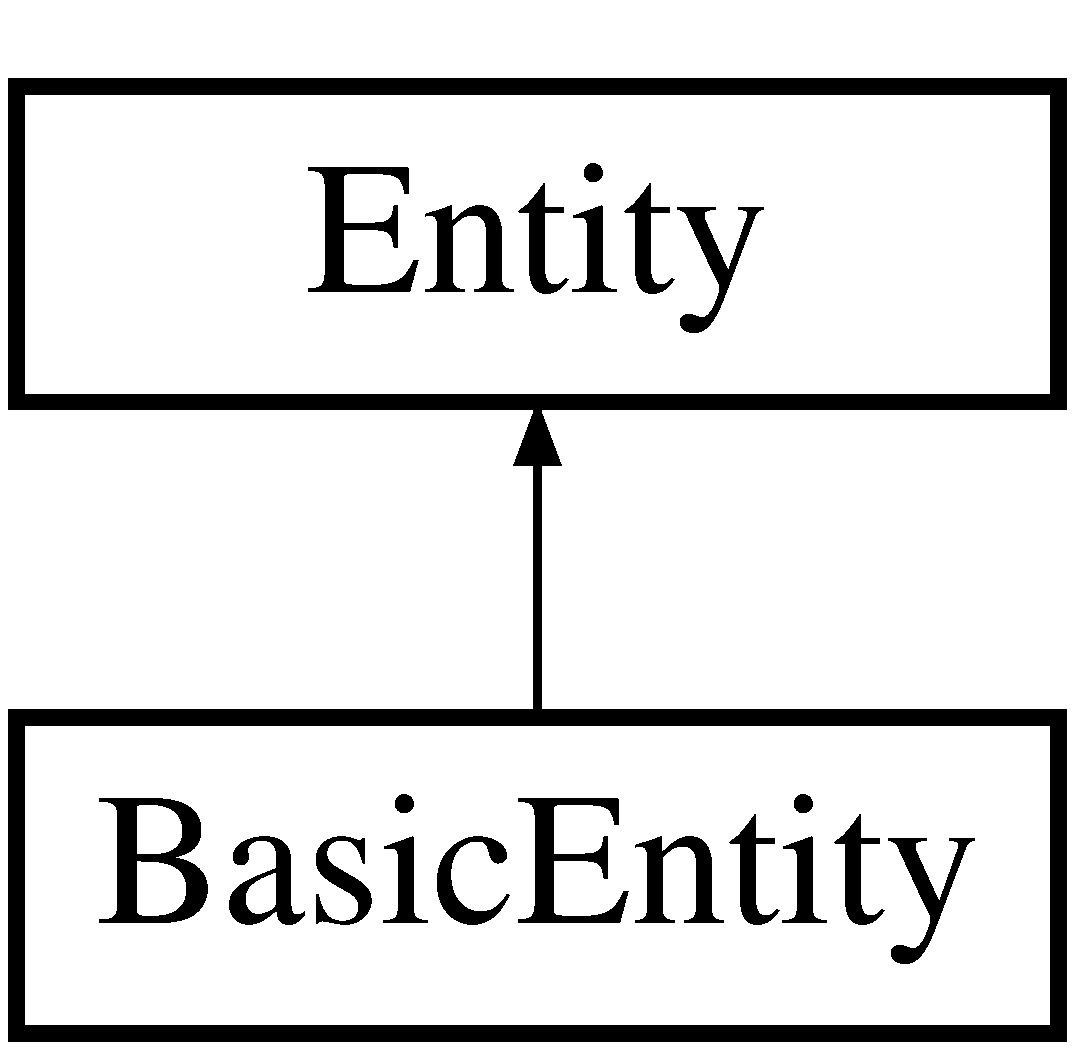
\includegraphics[height=2.000000cm]{class_basic_entity}
\end{center}
\end{figure}
\subsection*{Public Member Functions}
\begin{DoxyCompactItemize}
\item 
\hyperlink{class_basic_entity_a49c1b0069052d75862e215bf12bcb013}{Basic\+Entity} ()
\item 
\mbox{\Hypertarget{class_basic_entity_ac5113aef5520983d9939a9f3d01493eb}\label{class_basic_entity_ac5113aef5520983d9939a9f3d01493eb}} 
virtual void {\bfseries update} (float delta\+Time)
\end{DoxyCompactItemize}


\subsection{Detailed Description}
This file is part of a demo that shows how to use R\+T2D, a 2D Open\+GL framework.


\begin{DoxyItemize}
\item Copyright 2015 Rik Teerling \href{mailto:rik@onandoffables.com}{\tt rik@onandoffables.\+com}
\begin{DoxyItemize}
\item Initial commit 
\end{DoxyItemize}
\end{DoxyItemize}

\subsection{Constructor \& Destructor Documentation}
\mbox{\Hypertarget{class_basic_entity_a49c1b0069052d75862e215bf12bcb013}\label{class_basic_entity_a49c1b0069052d75862e215bf12bcb013}} 
\index{Basic\+Entity@{Basic\+Entity}!Basic\+Entity@{Basic\+Entity}}
\index{Basic\+Entity@{Basic\+Entity}!Basic\+Entity@{Basic\+Entity}}
\subsubsection{\texorpdfstring{Basic\+Entity()}{BasicEntity()}}
{\footnotesize\ttfamily Basic\+Entity\+::\+Basic\+Entity (\begin{DoxyParamCaption}{ }\end{DoxyParamCaption})}

This file is part of a demo that shows how to use R\+T2D, a 2D Open\+GL framework.


\begin{DoxyItemize}
\item Copyright 2015 Rik Teerling \href{mailto:rik@onandoffables.com}{\tt rik@onandoffables.\+com}
\begin{DoxyItemize}
\item Initial commit 
\end{DoxyItemize}
\end{DoxyItemize}

The documentation for this class was generated from the following files\+:\begin{DoxyCompactItemize}
\item 
basicentity.\+h\item 
basicentity.\+cpp\end{DoxyCompactItemize}

\hypertarget{struct_block}{}\section{Block Struct Reference}
\label{struct_block}\index{Block@{Block}}
\subsection*{Public Attributes}
\begin{DoxyCompactItemize}
\item 
\mbox{\Hypertarget{struct_block_aaa6a03a44f493a642f5254f45de02785}\label{struct_block_aaa6a03a44f493a642f5254f45de02785}} 
Point\+\_\+t$<$ int $>$ {\bfseries position}
\item 
\mbox{\Hypertarget{struct_block_a97a75574281e1a2a57fb6fd3fad16194}\label{struct_block_a97a75574281e1a2a57fb6fd3fad16194}} 
Point\+\_\+t$<$ int $>$ {\bfseries velocity}
\item 
\mbox{\Hypertarget{struct_block_a3ae5237a292637ddf5b2aa44e70a2325}\label{struct_block_a3ae5237a292637ddf5b2aa44e70a2325}} 
R\+G\+B\+A\+Color {\bfseries color}
\end{DoxyCompactItemize}


The documentation for this struct was generated from the following file\+:\begin{DoxyCompactItemize}
\item 
scene11.\+h\end{DoxyCompactItemize}

\hypertarget{class_boid}{}\section{Boid Class Reference}
\label{class_boid}\index{Boid@{Boid}}


{\ttfamily \#include $<$scene02.\+h$>$}

\subsection*{Public Member Functions}
\begin{DoxyCompactItemize}
\item 
\mbox{\Hypertarget{class_boid_abacc5b57737ab72b8fd0c2f6521d8f42}\label{class_boid_abacc5b57737ab72b8fd0c2f6521d8f42}} 
void {\bfseries update} (float delta\+Time)
\end{DoxyCompactItemize}
\subsection*{Public Attributes}
\begin{DoxyCompactItemize}
\item 
\mbox{\Hypertarget{class_boid_aa6455358e76571cdb7a05df210bc2d8c}\label{class_boid_aa6455358e76571cdb7a05df210bc2d8c}} 
Vector2 {\bfseries velocity}
\item 
\mbox{\Hypertarget{class_boid_afdfe88c3802c6d09072a5b19fde9eb8a}\label{class_boid_afdfe88c3802c6d09072a5b19fde9eb8a}} 
Point2 {\bfseries position}
\item 
\mbox{\Hypertarget{class_boid_aaa37997aae7557a214791420a652ebb7}\label{class_boid_aaa37997aae7557a214791420a652ebb7}} 
float {\bfseries rotation}
\item 
\mbox{\Hypertarget{class_boid_a8895ccc4eeddf79101a3ca2cf8c32eb7}\label{class_boid_a8895ccc4eeddf79101a3ca2cf8c32eb7}} 
Point2 {\bfseries scale}
\item 
\mbox{\Hypertarget{class_boid_a19e8b46421cfff55fe2b60ec9e13a478}\label{class_boid_a19e8b46421cfff55fe2b60ec9e13a478}} 
float {\bfseries waittime}
\item 
\mbox{\Hypertarget{class_boid_aa4f72fbe11f38833baba65af16f613b3}\label{class_boid_aa4f72fbe11f38833baba65af16f613b3}} 
Timer {\bfseries t}
\end{DoxyCompactItemize}


\subsection{Detailed Description}
This file is part of a demo that shows how to use R\+T2D, a 2D Open\+GL framework.


\begin{DoxyItemize}
\item Copyright 2015 Rik Teerling \href{mailto:rik@onandoffables.com}{\tt rik@onandoffables.\+com}
\begin{DoxyItemize}
\item Initial commit 
\end{DoxyItemize}
\end{DoxyItemize}

The documentation for this class was generated from the following file\+:\begin{DoxyCompactItemize}
\item 
scene02.\+h\end{DoxyCompactItemize}

\hypertarget{class_canvas}{}\section{Canvas Class Reference}
\label{class_canvas}\index{Canvas@{Canvas}}
Inheritance diagram for Canvas\+:\begin{figure}[H]
\begin{center}
\leavevmode
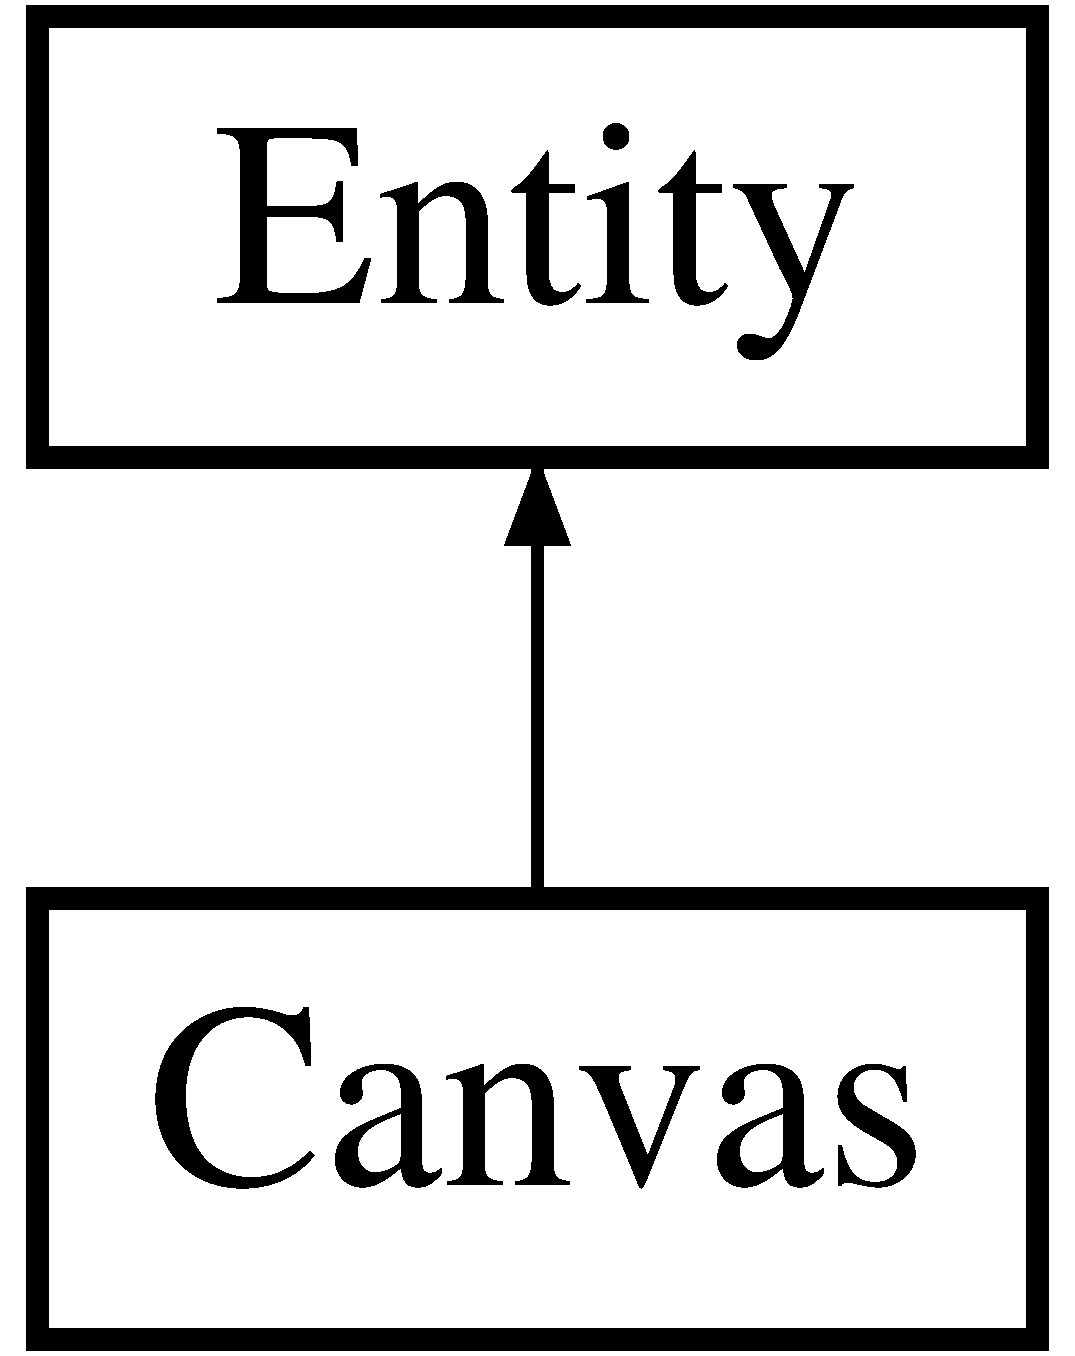
\includegraphics[height=2.000000cm]{class_canvas}
\end{center}
\end{figure}
\subsection*{Public Member Functions}
\begin{DoxyCompactItemize}
\item 
\hyperlink{class_canvas_a5fce53f080ad6540094901f9768805a8}{Canvas} ()
\item 
\mbox{\Hypertarget{class_canvas_a6b13d58b052c42d68e3d68a01cb8f6e9}\label{class_canvas_a6b13d58b052c42d68e3d68a01cb8f6e9}} 
{\bfseries Canvas} (int pixelsize)
\item 
\mbox{\Hypertarget{class_canvas_a20b219bfa7b0ccacf133f03e2d80764c}\label{class_canvas_a20b219bfa7b0ccacf133f03e2d80764c}} 
virtual void {\bfseries update} (float delta\+Time)
\item 
\mbox{\Hypertarget{class_canvas_a1395db675973b25403c93c86858ac980}\label{class_canvas_a1395db675973b25403c93c86858ac980}} 
void {\bfseries init} (int pixelsize)
\item 
\mbox{\Hypertarget{class_canvas_aeea330a891f999bd6524b66c07119f5c}\label{class_canvas_aeea330a891f999bd6524b66c07119f5c}} 
void {\bfseries set\+Pixel} (int x, int y, R\+G\+B\+A\+Color color)
\item 
\mbox{\Hypertarget{class_canvas_a50d5ab64f46ae2a098c9b4e4649ad9be}\label{class_canvas_a50d5ab64f46ae2a098c9b4e4649ad9be}} 
R\+G\+B\+A\+Color {\bfseries get\+Pixel} (int x, int y)
\item 
\mbox{\Hypertarget{class_canvas_ad95a8d64e5ccee7585ce950989e95221}\label{class_canvas_ad95a8d64e5ccee7585ce950989e95221}} 
void {\bfseries clear\+Pixel} (int x, int y)
\item 
\mbox{\Hypertarget{class_canvas_a9871b19d9a70e110ab1e009912de8c6d}\label{class_canvas_a9871b19d9a70e110ab1e009912de8c6d}} 
void {\bfseries fill} (R\+G\+B\+A\+Color color)
\item 
\mbox{\Hypertarget{class_canvas_afef4dc57abf127e369e004fe0d9a5597}\label{class_canvas_afef4dc57abf127e369e004fe0d9a5597}} 
int {\bfseries width} ()
\item 
\mbox{\Hypertarget{class_canvas_a515482fc400b41fc19954721d83d911e}\label{class_canvas_a515482fc400b41fc19954721d83d911e}} 
int {\bfseries height} ()
\item 
\mbox{\Hypertarget{class_canvas_a293a398441f5565747f49ea5582c71e7}\label{class_canvas_a293a398441f5565747f49ea5582c71e7}} 
void {\bfseries draw\+Sprite} (const \hyperlink{struct_pixel_sprite}{Pixel\+Sprite} \&spr)
\item 
\mbox{\Hypertarget{class_canvas_a56b0cb001187d6b1143b7fff2e3d262e}\label{class_canvas_a56b0cb001187d6b1143b7fff2e3d262e}} 
void {\bfseries clear\+Sprite} (const \hyperlink{struct_pixel_sprite}{Pixel\+Sprite} \&spr)
\end{DoxyCompactItemize}
\subsection*{Public Attributes}
\begin{DoxyCompactItemize}
\item 
\mbox{\Hypertarget{class_canvas_a8690c36b9534c872443b9df1acdc19f6}\label{class_canvas_a8690c36b9534c872443b9df1acdc19f6}} 
R\+G\+B\+A\+Color {\bfseries backgroundcolor}
\end{DoxyCompactItemize}


\subsection{Constructor \& Destructor Documentation}
\mbox{\Hypertarget{class_canvas_a5fce53f080ad6540094901f9768805a8}\label{class_canvas_a5fce53f080ad6540094901f9768805a8}} 
\index{Canvas@{Canvas}!Canvas@{Canvas}}
\index{Canvas@{Canvas}!Canvas@{Canvas}}
\subsubsection{\texorpdfstring{Canvas()}{Canvas()}}
{\footnotesize\ttfamily Canvas\+::\+Canvas (\begin{DoxyParamCaption}{ }\end{DoxyParamCaption})}

This file is part of a demo that shows how to use R\+T2D, a 2D Open\+GL framework.


\begin{DoxyItemize}
\item Copyright 2017 Rik Teerling \href{mailto:rik@onandoffables.com}{\tt rik@onandoffables.\+com}
\begin{DoxyItemize}
\item Initial commit 
\end{DoxyItemize}
\end{DoxyItemize}

The documentation for this class was generated from the following files\+:\begin{DoxyCompactItemize}
\item 
canvas.\+h\item 
canvas.\+cpp\end{DoxyCompactItemize}

\hypertarget{struct_cell}{}\section{Cell Struct Reference}
\label{struct_cell}\index{Cell@{Cell}}


{\ttfamily \#include $<$scene08.\+h$>$}

\subsection*{Public Attributes}
\begin{DoxyCompactItemize}
\item 
\mbox{\Hypertarget{struct_cell_accfbd18f0fa411f6183acd4117db87cb}\label{struct_cell_accfbd18f0fa411f6183acd4117db87cb}} 
\hyperlink{class_basic_entity}{Basic\+Entity} $\ast$ {\bfseries entity}
\item 
\mbox{\Hypertarget{struct_cell_a8e96c5ebe7be73e259c8de816273fe15}\label{struct_cell_a8e96c5ebe7be73e259c8de816273fe15}} 
Point\+\_\+t$<$ int $>$ {\bfseries position}
\end{DoxyCompactItemize}


\subsection{Detailed Description}
This file is part of a demo that shows how to use R\+T2D, a 2D Open\+GL framework.


\begin{DoxyItemize}
\item Copyright 2015 Rik Teerling \href{mailto:rik@onandoffables.com}{\tt rik@onandoffables.\+com}
\begin{DoxyItemize}
\item Initial commit 
\end{DoxyItemize}
\end{DoxyItemize}

The documentation for this struct was generated from the following file\+:\begin{DoxyCompactItemize}
\item 
scene08.\+h\end{DoxyCompactItemize}

\hypertarget{struct_field}{}\section{Field Struct Reference}
\label{struct_field}\index{Field@{Field}}


{\ttfamily \#include $<$scene14.\+h$>$}

\subsection*{Public Member Functions}
\begin{DoxyCompactItemize}
\item 
\mbox{\Hypertarget{struct_field_a63b8fdd184f4afe1adf143dbde54a57f}\label{struct_field_a63b8fdd184f4afe1adf143dbde54a57f}} 
void {\bfseries reset} ()
\end{DoxyCompactItemize}
\subsection*{Public Attributes}
\begin{DoxyCompactItemize}
\item 
\mbox{\Hypertarget{struct_field_aa5e55573ae91de84b5b2a824cacde3c9}\label{struct_field_aa5e55573ae91de84b5b2a824cacde3c9}} 
int {\bfseries fieldwidth} = 16
\item 
\mbox{\Hypertarget{struct_field_a2cac92d1bbaabf1fff016b26a5739844}\label{struct_field_a2cac92d1bbaabf1fff016b26a5739844}} 
int {\bfseries fieldheight} = 32
\item 
\mbox{\Hypertarget{struct_field_aa2e60e66a576bf6f5a447a476ebe2ec4}\label{struct_field_aa2e60e66a576bf6f5a447a476ebe2ec4}} 
std\+::vector$<$ \hyperlink{struct_pixel}{Pixel} $>$ {\bfseries cells}
\item 
\mbox{\Hypertarget{struct_field_a5d846e0822373c2635406a1ed90201d9}\label{struct_field_a5d846e0822373c2635406a1ed90201d9}} 
R\+G\+B\+A\+Color {\bfseries clearcolor} = R\+G\+B\+A\+Color(0,0,0,255)
\end{DoxyCompactItemize}


\subsection{Detailed Description}
This file is part of a demo that shows how to use R\+T2D, a 2D Open\+GL framework.


\begin{DoxyItemize}
\item Copyright 2017 Rik Teerling \href{mailto:rik@onandoffables.com}{\tt rik@onandoffables.\+com}
\begin{DoxyItemize}
\item Initial commit 
\end{DoxyItemize}
\end{DoxyItemize}

The documentation for this struct was generated from the following file\+:\begin{DoxyCompactItemize}
\item 
scene14.\+h\end{DoxyCompactItemize}

\hypertarget{struct_hex_field}{}\section{Hex\+Field Struct Reference}
\label{struct_hex_field}\index{Hex\+Field@{Hex\+Field}}


{\ttfamily \#include $<$scene06a.\+h$>$}

Inheritance diagram for Hex\+Field\+:\begin{figure}[H]
\begin{center}
\leavevmode
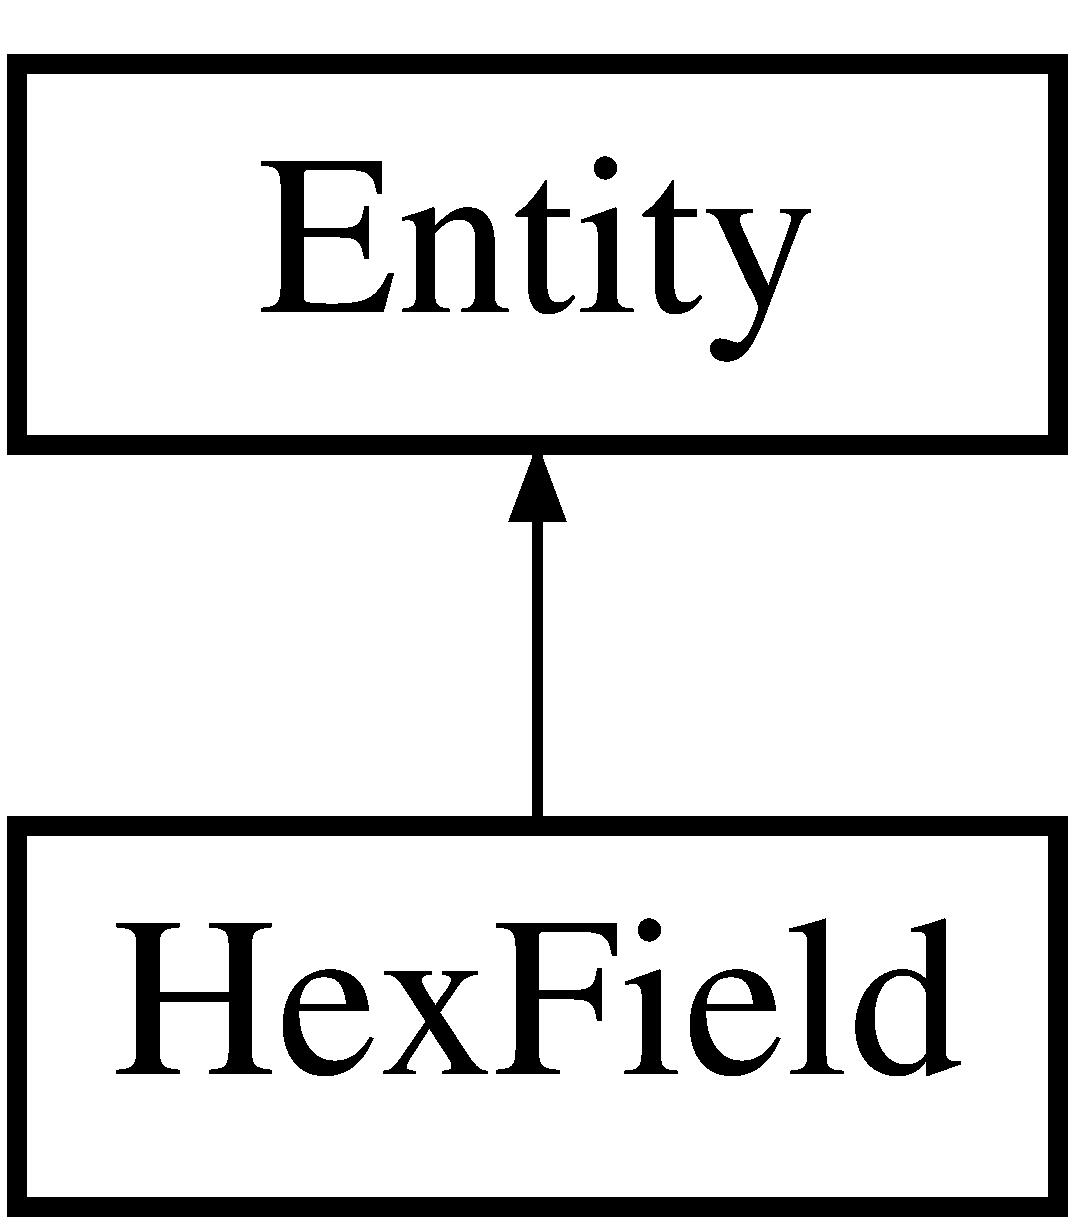
\includegraphics[height=2.000000cm]{struct_hex_field}
\end{center}
\end{figure}
\subsection*{Public Member Functions}
\begin{DoxyCompactItemize}
\item 
\mbox{\Hypertarget{struct_hex_field_a6199c5217338947bee4a23601894dabb}\label{struct_hex_field_a6199c5217338947bee4a23601894dabb}} 
virtual void {\bfseries update} (float delta\+Time)
\item 
\mbox{\Hypertarget{struct_hex_field_a3ee344d8d07e5c39cf69eeb76a397aa9}\label{struct_hex_field_a3ee344d8d07e5c39cf69eeb76a397aa9}} 
void {\bfseries setup\+Hex\+Grid} (const std\+::string \&filename, int u, int v, size\+\_\+t width, size\+\_\+t height, int r)
\item 
\mbox{\Hypertarget{struct_hex_field_a472962acbc5479f055ac82912f1b9f89}\label{struct_hex_field_a472962acbc5479f055ac82912f1b9f89}} 
size\+\_\+t {\bfseries findnearest} (Point2 pos)
\end{DoxyCompactItemize}
\subsection*{Public Attributes}
\begin{DoxyCompactItemize}
\item 
\mbox{\Hypertarget{struct_hex_field_a048e97d656dec37b3fc7765c004687b5}\label{struct_hex_field_a048e97d656dec37b3fc7765c004687b5}} 
size\+\_\+t {\bfseries cols}
\item 
\mbox{\Hypertarget{struct_hex_field_a0806894ce678db6f370eb53475e7a24a}\label{struct_hex_field_a0806894ce678db6f370eb53475e7a24a}} 
size\+\_\+t {\bfseries rows}
\item 
\mbox{\Hypertarget{struct_hex_field_a3ce28371f9ab4f575b64bfb2154b7415}\label{struct_hex_field_a3ce28371f9ab4f575b64bfb2154b7415}} 
int {\bfseries radius}
\end{DoxyCompactItemize}


\subsection{Detailed Description}
This file is part of a demo that shows how to use R\+T2D, a 2D Open\+GL framework.


\begin{DoxyItemize}
\item Copyright 2017 Rik Teerling \href{mailto:rik@onandoffables.com}{\tt rik@onandoffables.\+com}
\begin{DoxyItemize}
\item Initial commit 
\end{DoxyItemize}
\end{DoxyItemize}

The documentation for this struct was generated from the following file\+:\begin{DoxyCompactItemize}
\item 
scene06a.\+h\end{DoxyCompactItemize}

\hypertarget{struct_particle}{}\section{Particle Struct Reference}
\label{struct_particle}\index{Particle@{Particle}}


{\ttfamily \#include $<$scene07.\+h$>$}

\subsection*{Public Attributes}
\begin{DoxyCompactItemize}
\item 
\mbox{\Hypertarget{struct_particle_ad2a9bf68ebead1ca81e96ee1c36294d1}\label{struct_particle_ad2a9bf68ebead1ca81e96ee1c36294d1}} 
Point2 {\bfseries position}
\item 
\mbox{\Hypertarget{struct_particle_a37ff3cba1c5971f6933c262cd1c86edf}\label{struct_particle_a37ff3cba1c5971f6933c262cd1c86edf}} 
Vector2 {\bfseries velocity}
\item 
\mbox{\Hypertarget{struct_particle_af2d78dffc753c7faa80e91ad78c8d867}\label{struct_particle_af2d78dffc753c7faa80e91ad78c8d867}} 
R\+G\+B\+A\+Color {\bfseries color}
\end{DoxyCompactItemize}


\subsection{Detailed Description}
This file is part of a demo that shows how to use R\+T2D, a 2D Open\+GL framework.


\begin{DoxyItemize}
\item Copyright 2015 Rik Teerling \href{mailto:rik@onandoffables.com}{\tt rik@onandoffables.\+com}
\begin{DoxyItemize}
\item Initial commit 
\end{DoxyItemize}
\end{DoxyItemize}

The documentation for this struct was generated from the following file\+:\begin{DoxyCompactItemize}
\item 
scene07.\+h\end{DoxyCompactItemize}

\hypertarget{struct_pixel}{}\section{Pixel Struct Reference}
\label{struct_pixel}\index{Pixel@{Pixel}}


{\ttfamily \#include $<$canvas.\+h$>$}

\subsection*{Public Member Functions}
\begin{DoxyCompactItemize}
\item 
\mbox{\Hypertarget{struct_pixel_ac391c63d8fc2e5fd53eba7ef50947e3c}\label{struct_pixel_ac391c63d8fc2e5fd53eba7ef50947e3c}} 
{\bfseries Pixel} (Point\+\_\+t$<$ int $>$ pos, R\+G\+B\+A\+Color c)
\end{DoxyCompactItemize}
\subsection*{Public Attributes}
\begin{DoxyCompactItemize}
\item 
\mbox{\Hypertarget{struct_pixel_ae5a03b3f31635f11b67174b42a01fd40}\label{struct_pixel_ae5a03b3f31635f11b67174b42a01fd40}} 
Point\+\_\+t$<$ int $>$ {\bfseries position}
\item 
\mbox{\Hypertarget{struct_pixel_a035e2b936f417557664f69a06e32ed88}\label{struct_pixel_a035e2b936f417557664f69a06e32ed88}} 
R\+G\+B\+A\+Color {\bfseries color}
\end{DoxyCompactItemize}


\subsection{Detailed Description}
This file is part of a demo that shows how to use R\+T2D, a 2D Open\+GL framework.


\begin{DoxyItemize}
\item Copyright 2017 Rik Teerling \href{mailto:rik@onandoffables.com}{\tt rik@onandoffables.\+com}
\begin{DoxyItemize}
\item Initial commit 
\end{DoxyItemize}
\end{DoxyItemize}

The documentation for this struct was generated from the following file\+:\begin{DoxyCompactItemize}
\item 
canvas.\+h\end{DoxyCompactItemize}

\hypertarget{struct_pixel_sprite}{}\section{Pixel\+Sprite Struct Reference}
\label{struct_pixel_sprite}\index{Pixel\+Sprite@{Pixel\+Sprite}}
\subsection*{Public Member Functions}
\begin{DoxyCompactItemize}
\item 
\mbox{\Hypertarget{struct_pixel_sprite_a1a08e75f84e62a8d41d9167995e1b633}\label{struct_pixel_sprite_a1a08e75f84e62a8d41d9167995e1b633}} 
void {\bfseries init} (char $\ast$data, int w, int h)
\item 
\mbox{\Hypertarget{struct_pixel_sprite_a478a35c777092340f307df5a5c886025}\label{struct_pixel_sprite_a478a35c777092340f307df5a5c886025}} 
\hyperlink{struct_pixel_sprite}{Pixel\+Sprite} {\bfseries rotation} (float a)
\end{DoxyCompactItemize}
\subsection*{Public Attributes}
\begin{DoxyCompactItemize}
\item 
\mbox{\Hypertarget{struct_pixel_sprite_a33f8864f6d53108c5582256a70bd545a}\label{struct_pixel_sprite_a33f8864f6d53108c5582256a70bd545a}} 
std\+::vector$<$ \hyperlink{struct_pixel}{Pixel} $>$ {\bfseries pixels}
\item 
\mbox{\Hypertarget{struct_pixel_sprite_a8b952793f8ea74335359a37c3174278c}\label{struct_pixel_sprite_a8b952793f8ea74335359a37c3174278c}} 
Point\+\_\+t$<$ int $>$ {\bfseries position}
\item 
R\+G\+B\+A\+Color {\bfseries pallete} \mbox{[}10\mbox{]}
\end{DoxyCompactItemize}


\subsection{Member Data Documentation}
\mbox{\Hypertarget{struct_pixel_sprite_a58b79eb36d8b9caba9a4d15d178ac6bb}\label{struct_pixel_sprite_a58b79eb36d8b9caba9a4d15d178ac6bb}} 
\index{Pixel\+Sprite@{Pixel\+Sprite}!pallete@{pallete}}
\index{pallete@{pallete}!Pixel\+Sprite@{Pixel\+Sprite}}
\subsubsection{\texorpdfstring{pallete}{pallete}}
{\footnotesize\ttfamily R\+G\+B\+A\+Color Pixel\+Sprite\+::pallete\mbox{[}10\mbox{]}}

{\bfseries Initial value\+:}
\begin{DoxyCode}
= \{
        MAGENTA, 
        WHITE,
        BLUE,
        MAGENTA,
        RED,
        GREEN,
        YELLOW,
        PINK,
        ORANGE,
        GRAY
    \}
\end{DoxyCode}


The documentation for this struct was generated from the following file\+:\begin{DoxyCompactItemize}
\item 
canvas.\+h\end{DoxyCompactItemize}

\hypertarget{struct_player}{}\section{Player Struct Reference}
\label{struct_player}\index{Player@{Player}}


{\ttfamily \#include $<$superscene.\+h$>$}

\subsection*{Public Attributes}
\begin{DoxyCompactItemize}
\item 
\mbox{\Hypertarget{struct_player_a74db0ea8732ec5ab3f1575798af3aa1a}\label{struct_player_a74db0ea8732ec5ab3f1575798af3aa1a}} 
int {\bfseries mouseclicks} = 0
\end{DoxyCompactItemize}


\subsection{Detailed Description}
This file is part of a demo that shows how to use R\+T2D, a 2D Open\+GL framework.


\begin{DoxyItemize}
\item Copyright 2015 Rik Teerling \href{mailto:rik@onandoffables.com}{\tt rik@onandoffables.\+com}
\begin{DoxyItemize}
\item Initial commit 
\end{DoxyItemize}
\end{DoxyItemize}

The documentation for this struct was generated from the following file\+:\begin{DoxyCompactItemize}
\item 
superscene.\+h\end{DoxyCompactItemize}

\hypertarget{class_scene00}{}\section{Scene00 Class Reference}
\label{class_scene00}\index{Scene00@{Scene00}}


{\ttfamily \#include $<$scene00.\+h$>$}

Inheritance diagram for Scene00\+:\begin{figure}[H]
\begin{center}
\leavevmode
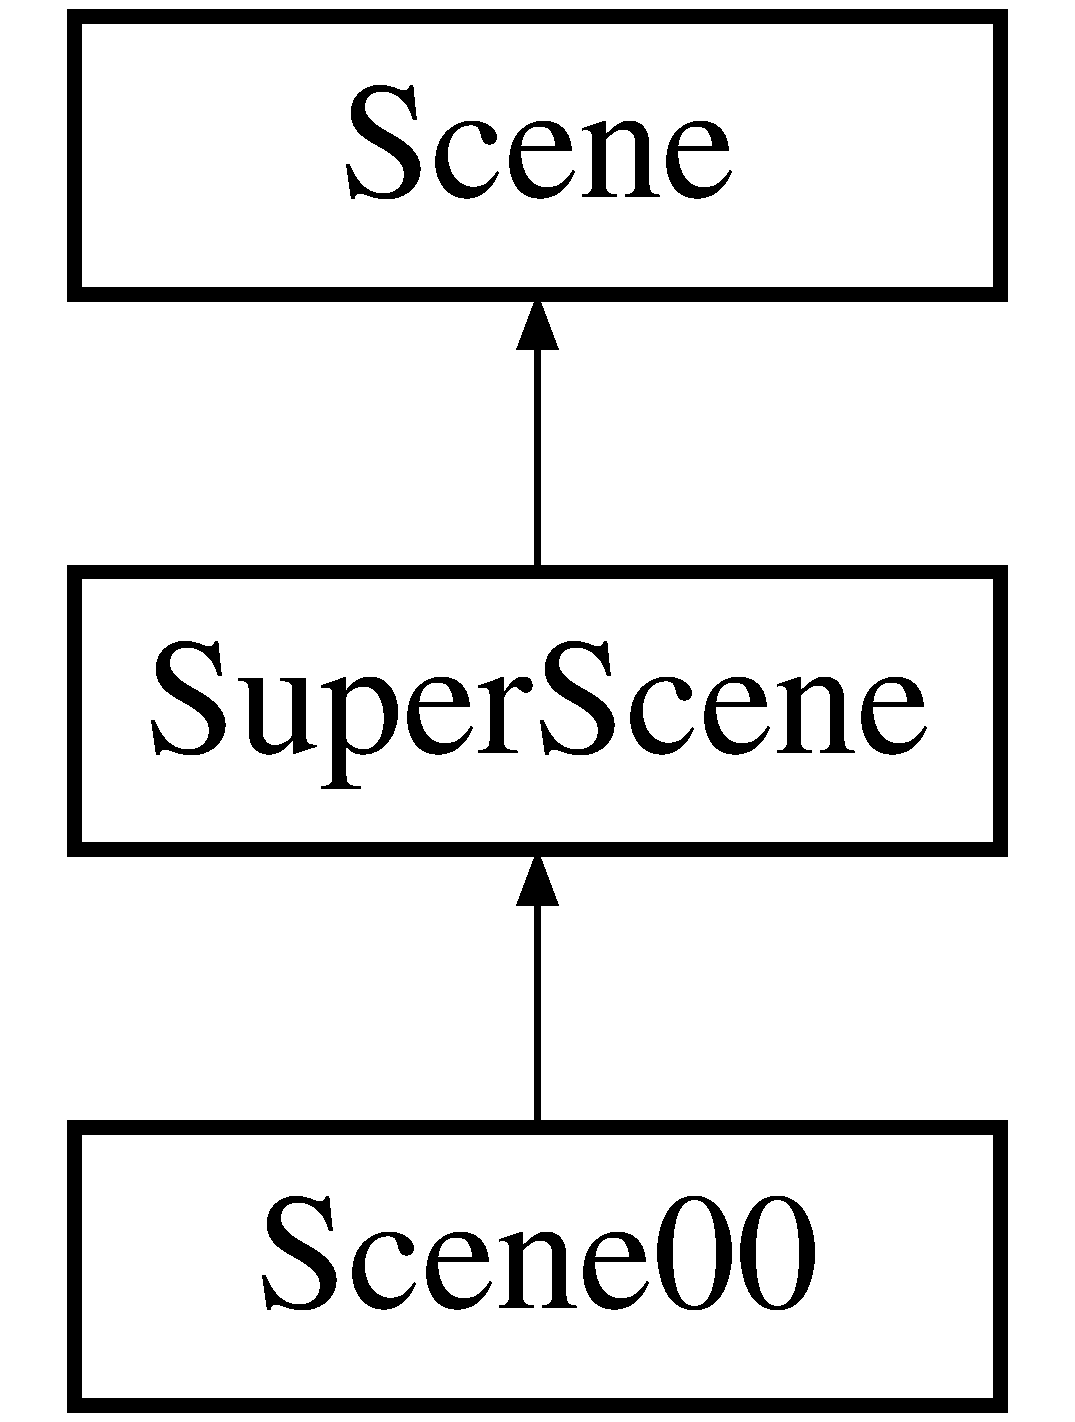
\includegraphics[height=3.000000cm]{class_scene00}
\end{center}
\end{figure}
\subsection*{Public Member Functions}
\begin{DoxyCompactItemize}
\item 
\hyperlink{class_scene00_acf63b43edc4b904b0d94e7aa94cc2c3b}{Scene00} ()
\item 
\mbox{\Hypertarget{class_scene00_aedbfa6b7ccb804ec37869b8e469bb8ad}\label{class_scene00_aedbfa6b7ccb804ec37869b8e469bb8ad}} 
virtual void {\bfseries update} (float delta\+Time)
\end{DoxyCompactItemize}
\subsection*{Additional Inherited Members}


\subsection{Detailed Description}
This file is part of a demo that shows how to use R\+T2D, a 2D Open\+GL framework.


\begin{DoxyItemize}
\item Copyright 2015 Rik Teerling \href{mailto:rik@onandoffables.com}{\tt rik@onandoffables.\+com}
\begin{DoxyItemize}
\item Initial commit 
\end{DoxyItemize}
\end{DoxyItemize}

\subsection{Constructor \& Destructor Documentation}
\mbox{\Hypertarget{class_scene00_acf63b43edc4b904b0d94e7aa94cc2c3b}\label{class_scene00_acf63b43edc4b904b0d94e7aa94cc2c3b}} 
\index{Scene00@{Scene00}!Scene00@{Scene00}}
\index{Scene00@{Scene00}!Scene00@{Scene00}}
\subsubsection{\texorpdfstring{Scene00()}{Scene00()}}
{\footnotesize\ttfamily Scene00\+::\+Scene00 (\begin{DoxyParamCaption}{ }\end{DoxyParamCaption})}

This file is part of a demo that shows how to use R\+T2D, a 2D Open\+GL framework.


\begin{DoxyItemize}
\item Copyright 2015 Rik Teerling \href{mailto:rik@onandoffables.com}{\tt rik@onandoffables.\+com}
\begin{DoxyItemize}
\item Initial commit 
\end{DoxyItemize}
\end{DoxyItemize}

The documentation for this class was generated from the following files\+:\begin{DoxyCompactItemize}
\item 
scene00.\+h\item 
scene00.\+cpp\end{DoxyCompactItemize}

\hypertarget{class_scene01}{}\section{Scene01 Class Reference}
\label{class_scene01}\index{Scene01@{Scene01}}


{\ttfamily \#include $<$scene01.\+h$>$}

Inheritance diagram for Scene01\+:\begin{figure}[H]
\begin{center}
\leavevmode
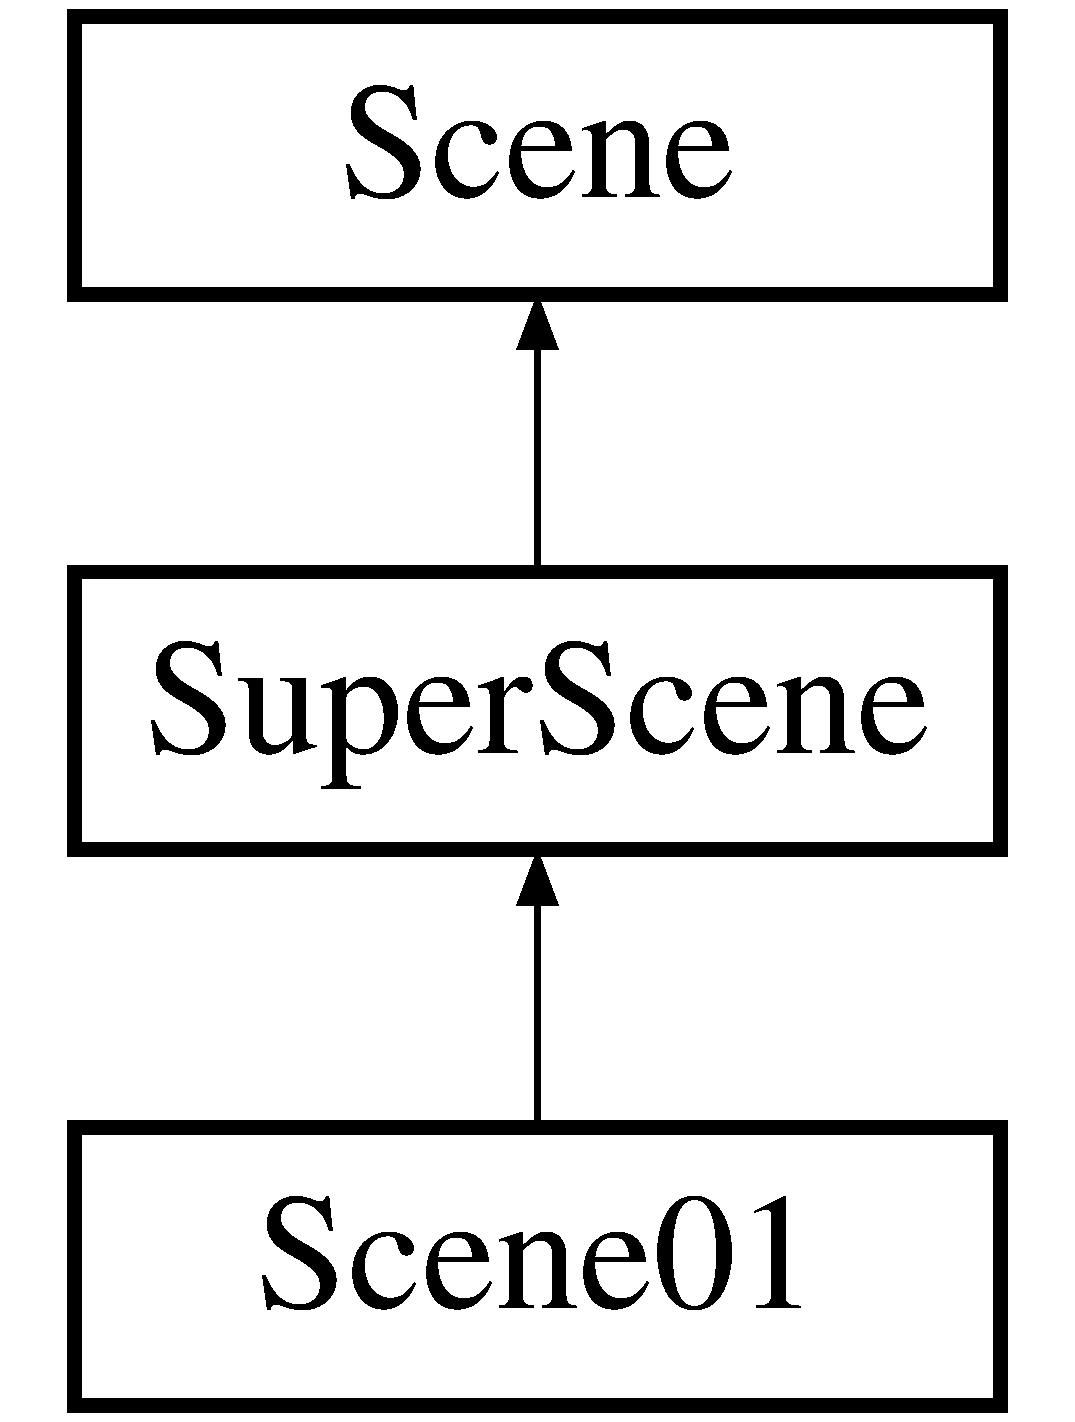
\includegraphics[height=3.000000cm]{class_scene01}
\end{center}
\end{figure}
\subsection*{Public Member Functions}
\begin{DoxyCompactItemize}
\item 
\hyperlink{class_scene01_aa485d27ddea0a312ce76a36f18417b93}{Scene01} ()
\item 
\mbox{\Hypertarget{class_scene01_a8ce3d409ab61628aadeb26202d1686f7}\label{class_scene01_a8ce3d409ab61628aadeb26202d1686f7}} 
virtual void {\bfseries update} (float delta\+Time)
\end{DoxyCompactItemize}
\subsection*{Additional Inherited Members}


\subsection{Detailed Description}
This file is part of a demo that shows how to use R\+T2D, a 2D Open\+GL framework.


\begin{DoxyItemize}
\item Copyright 2015 Rik Teerling \href{mailto:rik@onandoffables.com}{\tt rik@onandoffables.\+com}
\begin{DoxyItemize}
\item Initial commit 
\end{DoxyItemize}
\end{DoxyItemize}

\subsection{Constructor \& Destructor Documentation}
\mbox{\Hypertarget{class_scene01_aa485d27ddea0a312ce76a36f18417b93}\label{class_scene01_aa485d27ddea0a312ce76a36f18417b93}} 
\index{Scene01@{Scene01}!Scene01@{Scene01}}
\index{Scene01@{Scene01}!Scene01@{Scene01}}
\subsubsection{\texorpdfstring{Scene01()}{Scene01()}}
{\footnotesize\ttfamily Scene01\+::\+Scene01 (\begin{DoxyParamCaption}{ }\end{DoxyParamCaption})}

This file is part of a demo that shows how to use R\+T2D, a 2D Open\+GL framework.


\begin{DoxyItemize}
\item Copyright 2015 Rik Teerling \href{mailto:rik@onandoffables.com}{\tt rik@onandoffables.\+com}
\begin{DoxyItemize}
\item Initial commit 
\end{DoxyItemize}
\end{DoxyItemize}

The documentation for this class was generated from the following files\+:\begin{DoxyCompactItemize}
\item 
scene01.\+h\item 
scene01.\+cpp\end{DoxyCompactItemize}

\hypertarget{class_scene02}{}\section{Scene02 Class Reference}
\label{class_scene02}\index{Scene02@{Scene02}}
Inheritance diagram for Scene02\+:\begin{figure}[H]
\begin{center}
\leavevmode
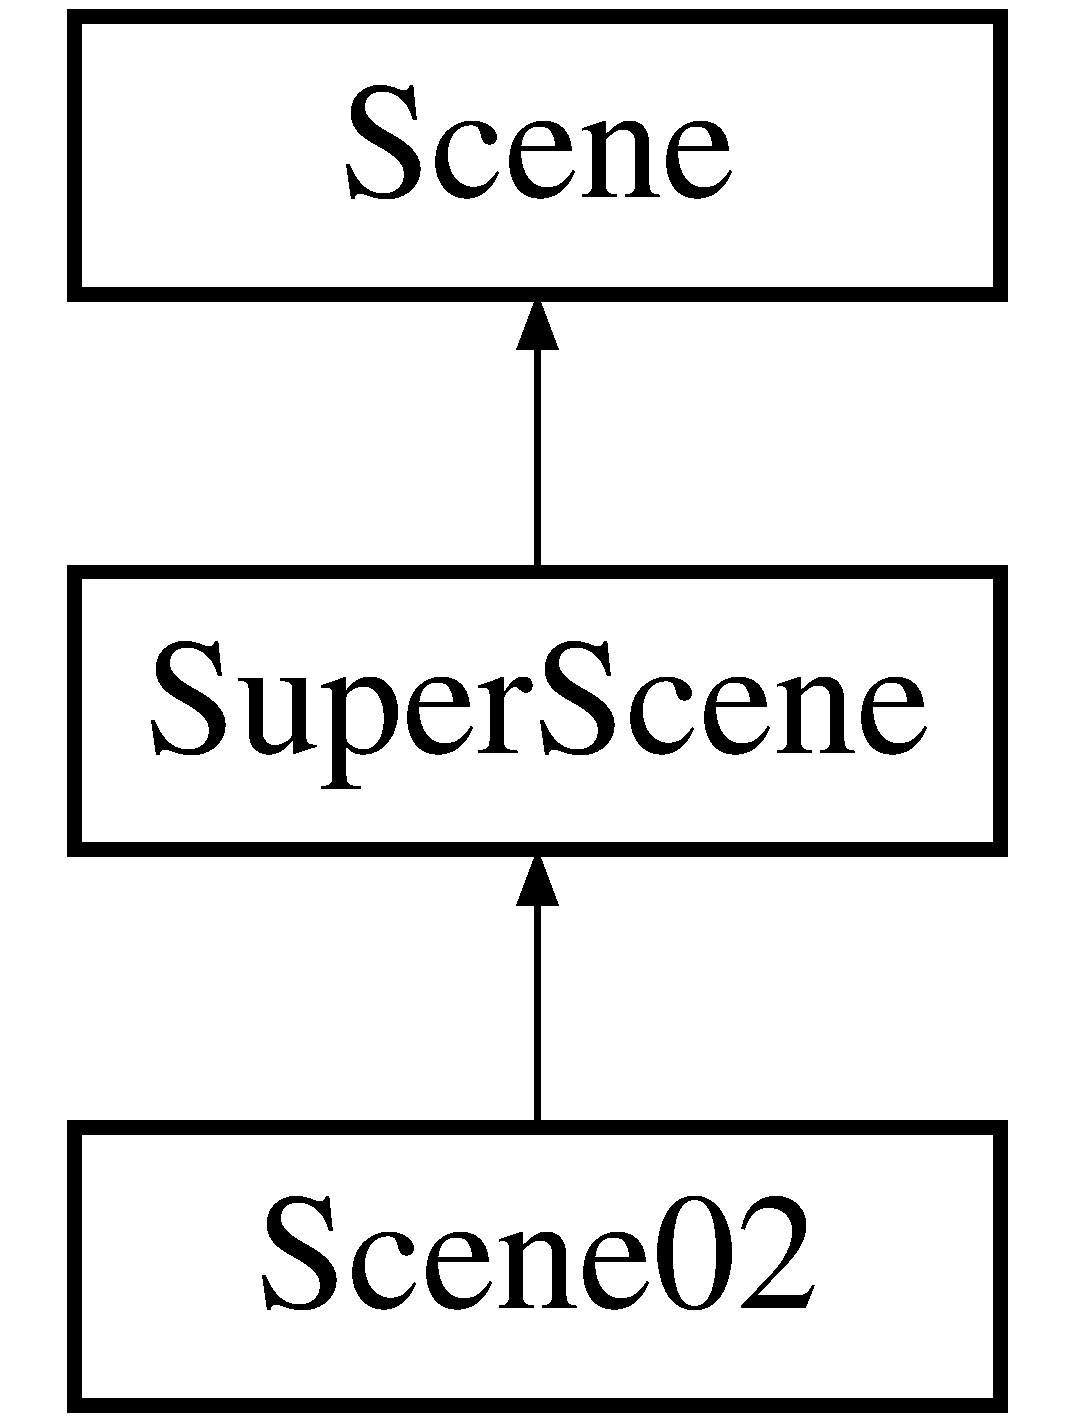
\includegraphics[height=3.000000cm]{class_scene02}
\end{center}
\end{figure}
\subsection*{Public Member Functions}
\begin{DoxyCompactItemize}
\item 
\hyperlink{class_scene02_a961d6fa8c7dddc46ad13959d864ff332}{Scene02} ()
\item 
\mbox{\Hypertarget{class_scene02_af02675b877854ee94598058b0e48f042}\label{class_scene02_af02675b877854ee94598058b0e48f042}} 
virtual void {\bfseries update} (float delta\+Time)
\end{DoxyCompactItemize}
\subsection*{Additional Inherited Members}


\subsection{Constructor \& Destructor Documentation}
\mbox{\Hypertarget{class_scene02_a961d6fa8c7dddc46ad13959d864ff332}\label{class_scene02_a961d6fa8c7dddc46ad13959d864ff332}} 
\index{Scene02@{Scene02}!Scene02@{Scene02}}
\index{Scene02@{Scene02}!Scene02@{Scene02}}
\subsubsection{\texorpdfstring{Scene02()}{Scene02()}}
{\footnotesize\ttfamily Scene02\+::\+Scene02 (\begin{DoxyParamCaption}{ }\end{DoxyParamCaption})}

This file is part of a demo that shows how to use R\+T2D, a 2D Open\+GL framework.


\begin{DoxyItemize}
\item Copyright 2015 Rik Teerling \href{mailto:rik@onandoffables.com}{\tt rik@onandoffables.\+com}
\begin{DoxyItemize}
\item Initial commit 
\end{DoxyItemize}
\end{DoxyItemize}

The documentation for this class was generated from the following files\+:\begin{DoxyCompactItemize}
\item 
scene02.\+h\item 
scene02.\+cpp\end{DoxyCompactItemize}

\hypertarget{class_scene03}{}\section{Scene03 Class Reference}
\label{class_scene03}\index{Scene03@{Scene03}}


{\ttfamily \#include $<$scene03.\+h$>$}

Inheritance diagram for Scene03\+:\begin{figure}[H]
\begin{center}
\leavevmode
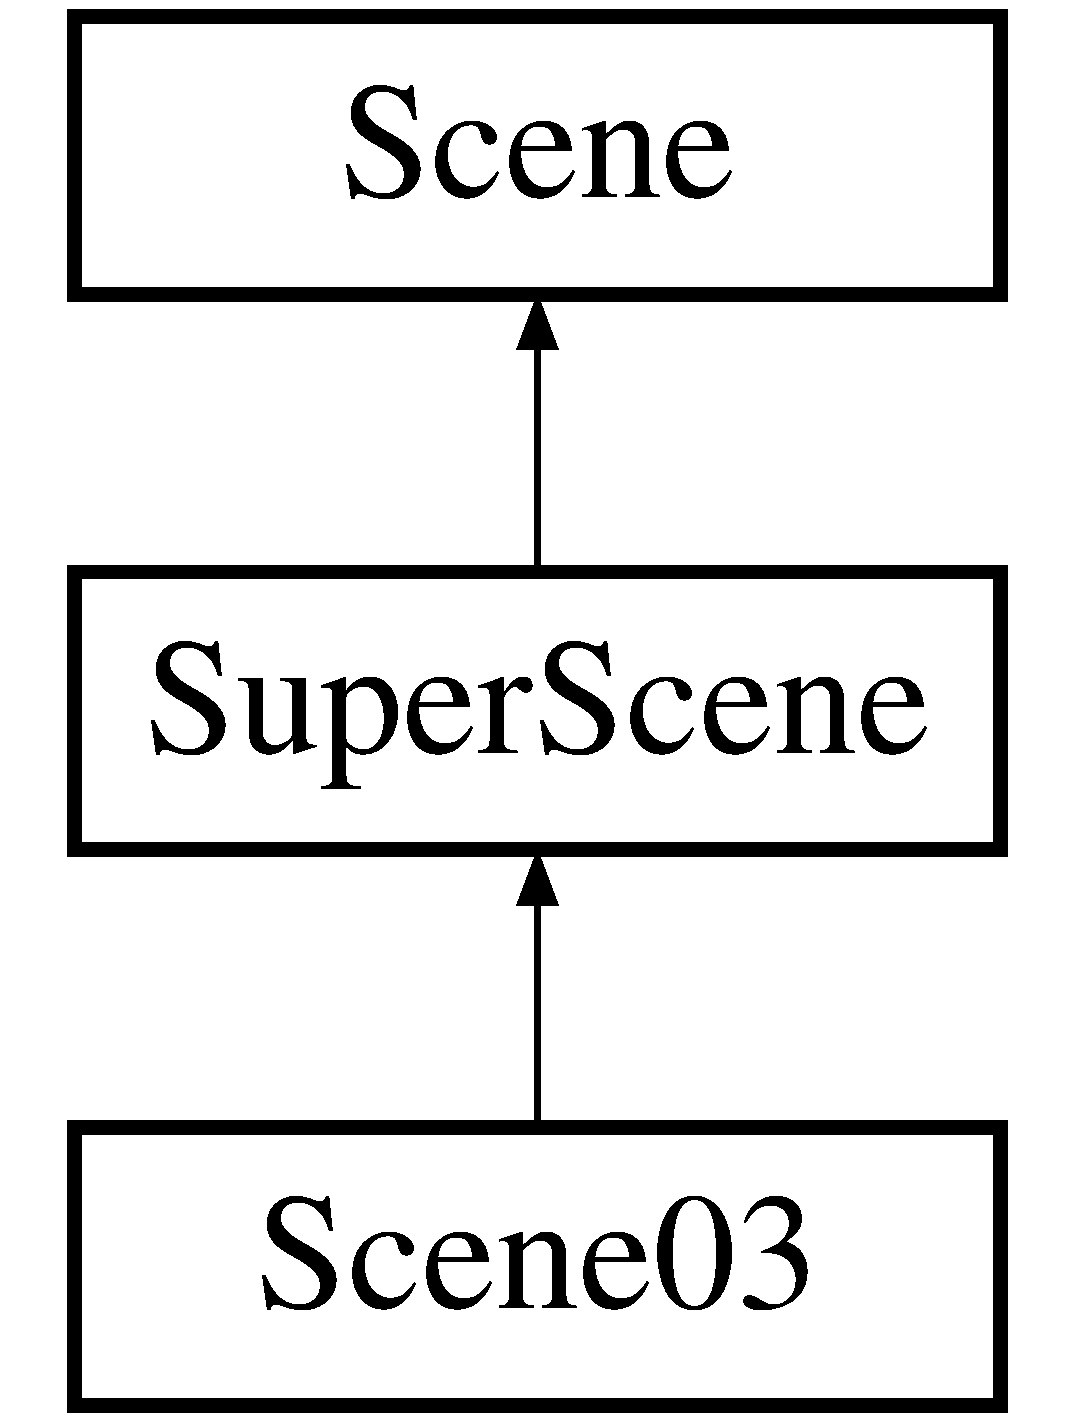
\includegraphics[height=3.000000cm]{class_scene03}
\end{center}
\end{figure}
\subsection*{Public Member Functions}
\begin{DoxyCompactItemize}
\item 
\mbox{\Hypertarget{class_scene03_a7f1ee2ee37db860eb64a418726f73e82}\label{class_scene03_a7f1ee2ee37db860eb64a418726f73e82}} 
virtual void {\bfseries update} (float delta\+Time)
\end{DoxyCompactItemize}
\subsection*{Additional Inherited Members}


\subsection{Detailed Description}
This file is part of a demo that shows how to use R\+T2D, a 2D Open\+GL framework.


\begin{DoxyItemize}
\item Copyright 2015 Rik Teerling \href{mailto:rik@onandoffables.com}{\tt rik@onandoffables.\+com}
\begin{DoxyItemize}
\item Initial commit 
\end{DoxyItemize}
\end{DoxyItemize}

The documentation for this class was generated from the following files\+:\begin{DoxyCompactItemize}
\item 
scene03.\+h\item 
scene03.\+cpp\end{DoxyCompactItemize}

\hypertarget{class_scene03a}{}\section{Scene03a Class Reference}
\label{class_scene03a}\index{Scene03a@{Scene03a}}


{\ttfamily \#include $<$scene03a.\+h$>$}

Inheritance diagram for Scene03a\+:\begin{figure}[H]
\begin{center}
\leavevmode
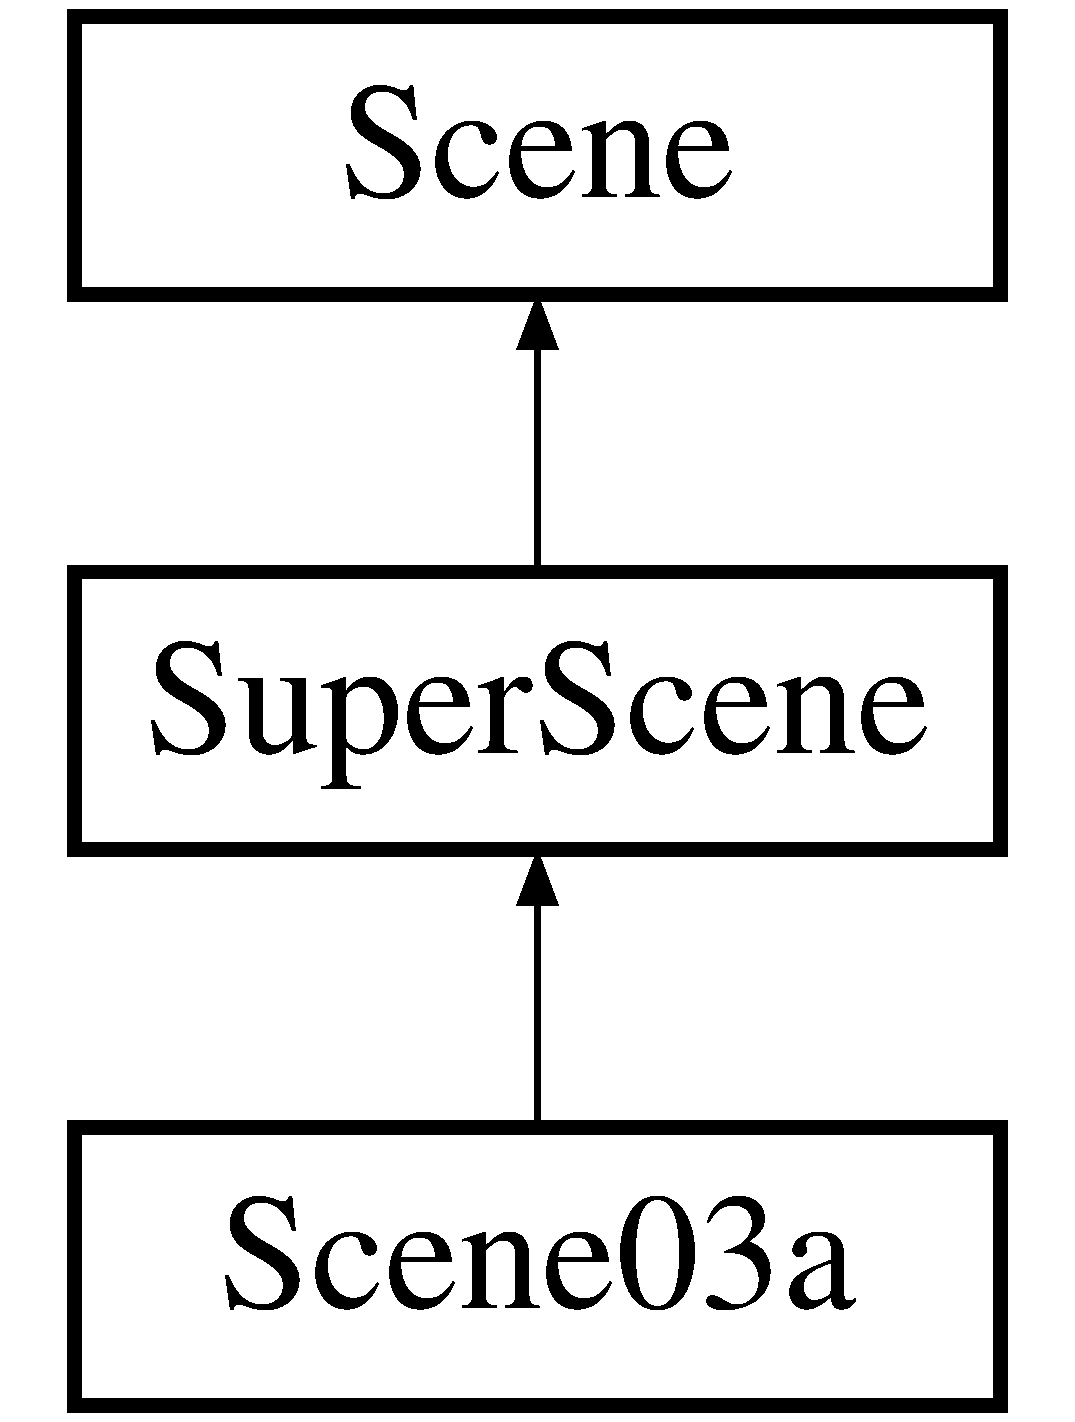
\includegraphics[height=3.000000cm]{class_scene03a}
\end{center}
\end{figure}
\subsection*{Public Member Functions}
\begin{DoxyCompactItemize}
\item 
\hyperlink{class_scene03a_a51e76ff839b9e5aa276aee0a5ca1b137}{Scene03a} ()
\item 
\mbox{\Hypertarget{class_scene03a_a96d705875f379a21b342358a3aa814a2}\label{class_scene03a_a96d705875f379a21b342358a3aa814a2}} 
virtual void {\bfseries update} (float delta\+Time)
\end{DoxyCompactItemize}
\subsection*{Additional Inherited Members}


\subsection{Detailed Description}
This file is part of a demo that shows how to use R\+T2D, a 2D Open\+GL framework.


\begin{DoxyItemize}
\item Copyright 2015 Rik Teerling \href{mailto:rik@onandoffables.com}{\tt rik@onandoffables.\+com}
\begin{DoxyItemize}
\item Initial commit 
\end{DoxyItemize}
\end{DoxyItemize}

\subsection{Constructor \& Destructor Documentation}
\mbox{\Hypertarget{class_scene03a_a51e76ff839b9e5aa276aee0a5ca1b137}\label{class_scene03a_a51e76ff839b9e5aa276aee0a5ca1b137}} 
\index{Scene03a@{Scene03a}!Scene03a@{Scene03a}}
\index{Scene03a@{Scene03a}!Scene03a@{Scene03a}}
\subsubsection{\texorpdfstring{Scene03a()}{Scene03a()}}
{\footnotesize\ttfamily Scene03a\+::\+Scene03a (\begin{DoxyParamCaption}{ }\end{DoxyParamCaption})}

This file is part of a demo that shows how to use R\+T2D, a 2D Open\+GL framework.


\begin{DoxyItemize}
\item Copyright 2015 Rik Teerling \href{mailto:rik@onandoffables.com}{\tt rik@onandoffables.\+com}
\begin{DoxyItemize}
\item Initial commit 
\end{DoxyItemize}
\end{DoxyItemize}

The documentation for this class was generated from the following files\+:\begin{DoxyCompactItemize}
\item 
scene03a.\+h\item 
scene03a.\+cpp\end{DoxyCompactItemize}

\hypertarget{class_scene03b}{}\section{Scene03b Class Reference}
\label{class_scene03b}\index{Scene03b@{Scene03b}}


{\ttfamily \#include $<$scene03b.\+h$>$}

Inheritance diagram for Scene03b\+:\begin{figure}[H]
\begin{center}
\leavevmode
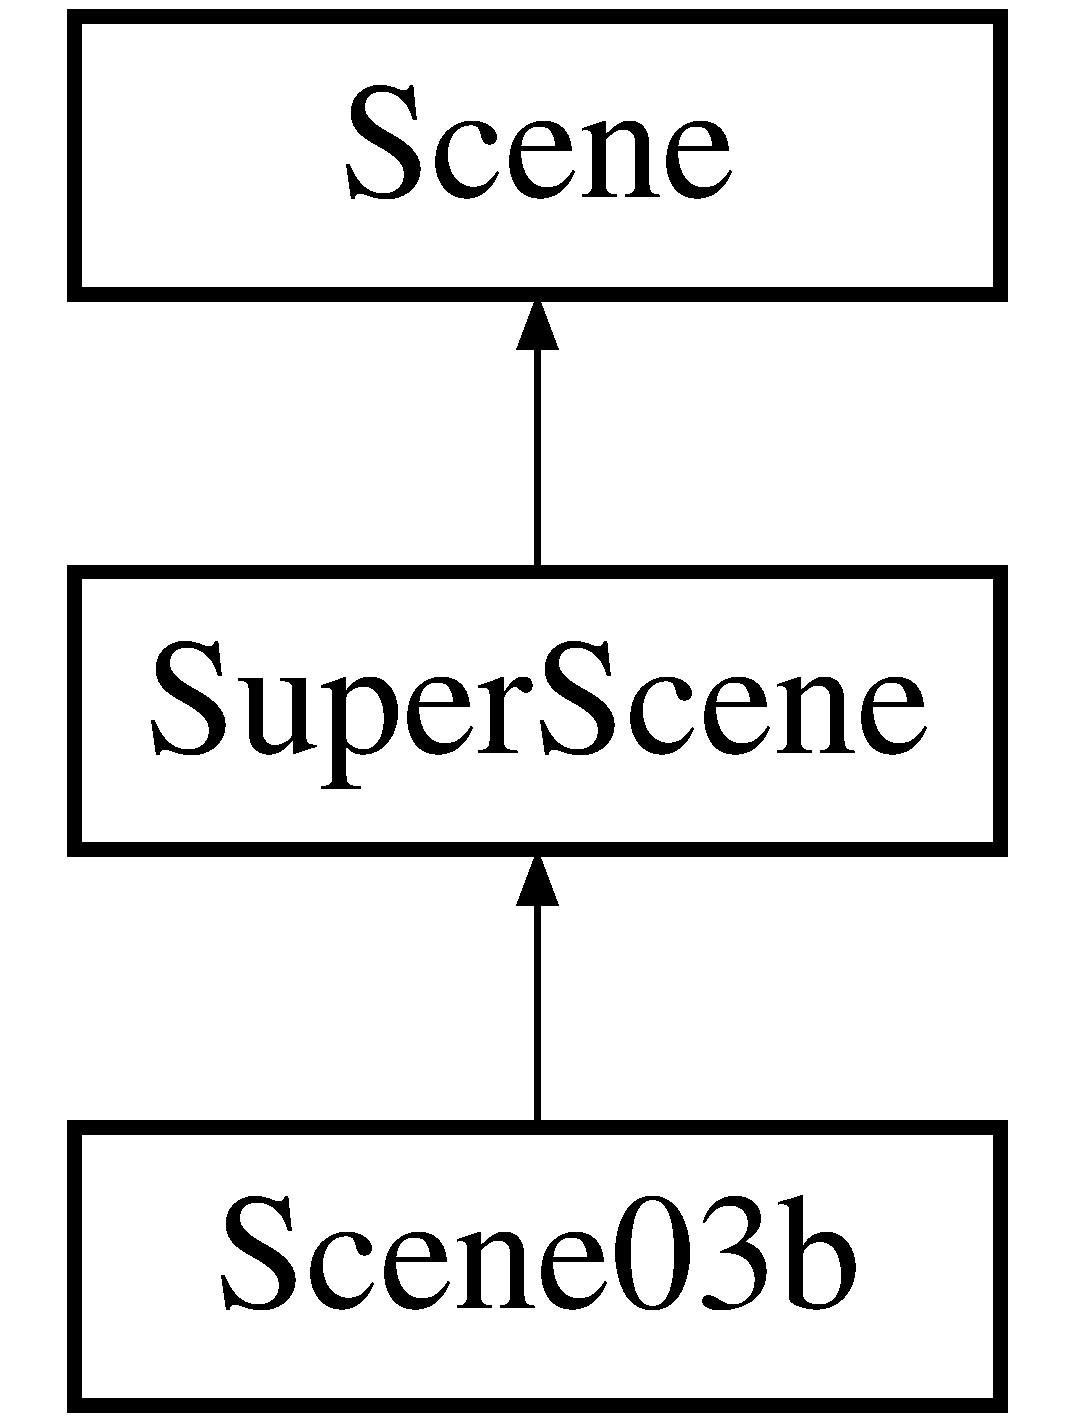
\includegraphics[height=3.000000cm]{class_scene03b}
\end{center}
\end{figure}
\subsection*{Public Member Functions}
\begin{DoxyCompactItemize}
\item 
\hyperlink{class_scene03b_a24f82c7664305aeeaeb86ffd681d6a3f}{Scene03b} ()
\item 
\mbox{\Hypertarget{class_scene03b_abdb8e9b90007a61b4b385a777dc51779}\label{class_scene03b_abdb8e9b90007a61b4b385a777dc51779}} 
virtual void {\bfseries update} (float delta\+Time)
\end{DoxyCompactItemize}
\subsection*{Additional Inherited Members}


\subsection{Detailed Description}
This file is part of a demo that shows how to use R\+T2D, a 2D Open\+GL framework.


\begin{DoxyItemize}
\item Copyright 2015 Rik Teerling \href{mailto:rik@onandoffables.com}{\tt rik@onandoffables.\+com}
\begin{DoxyItemize}
\item Initial commit 
\end{DoxyItemize}
\end{DoxyItemize}

\subsection{Constructor \& Destructor Documentation}
\mbox{\Hypertarget{class_scene03b_a24f82c7664305aeeaeb86ffd681d6a3f}\label{class_scene03b_a24f82c7664305aeeaeb86ffd681d6a3f}} 
\index{Scene03b@{Scene03b}!Scene03b@{Scene03b}}
\index{Scene03b@{Scene03b}!Scene03b@{Scene03b}}
\subsubsection{\texorpdfstring{Scene03b()}{Scene03b()}}
{\footnotesize\ttfamily Scene03b\+::\+Scene03b (\begin{DoxyParamCaption}{ }\end{DoxyParamCaption})}

This file is part of a demo that shows how to use R\+T2D, a 2D Open\+GL framework.


\begin{DoxyItemize}
\item Copyright 2015 Rik Teerling \href{mailto:rik@onandoffables.com}{\tt rik@onandoffables.\+com}
\begin{DoxyItemize}
\item Initial commit 
\end{DoxyItemize}
\end{DoxyItemize}

The documentation for this class was generated from the following files\+:\begin{DoxyCompactItemize}
\item 
scene03b.\+h\item 
scene03b.\+cpp\end{DoxyCompactItemize}

\hypertarget{class_scene04}{}\section{Scene04 Class Reference}
\label{class_scene04}\index{Scene04@{Scene04}}


{\ttfamily \#include $<$scene04.\+h$>$}

Inheritance diagram for Scene04\+:\begin{figure}[H]
\begin{center}
\leavevmode
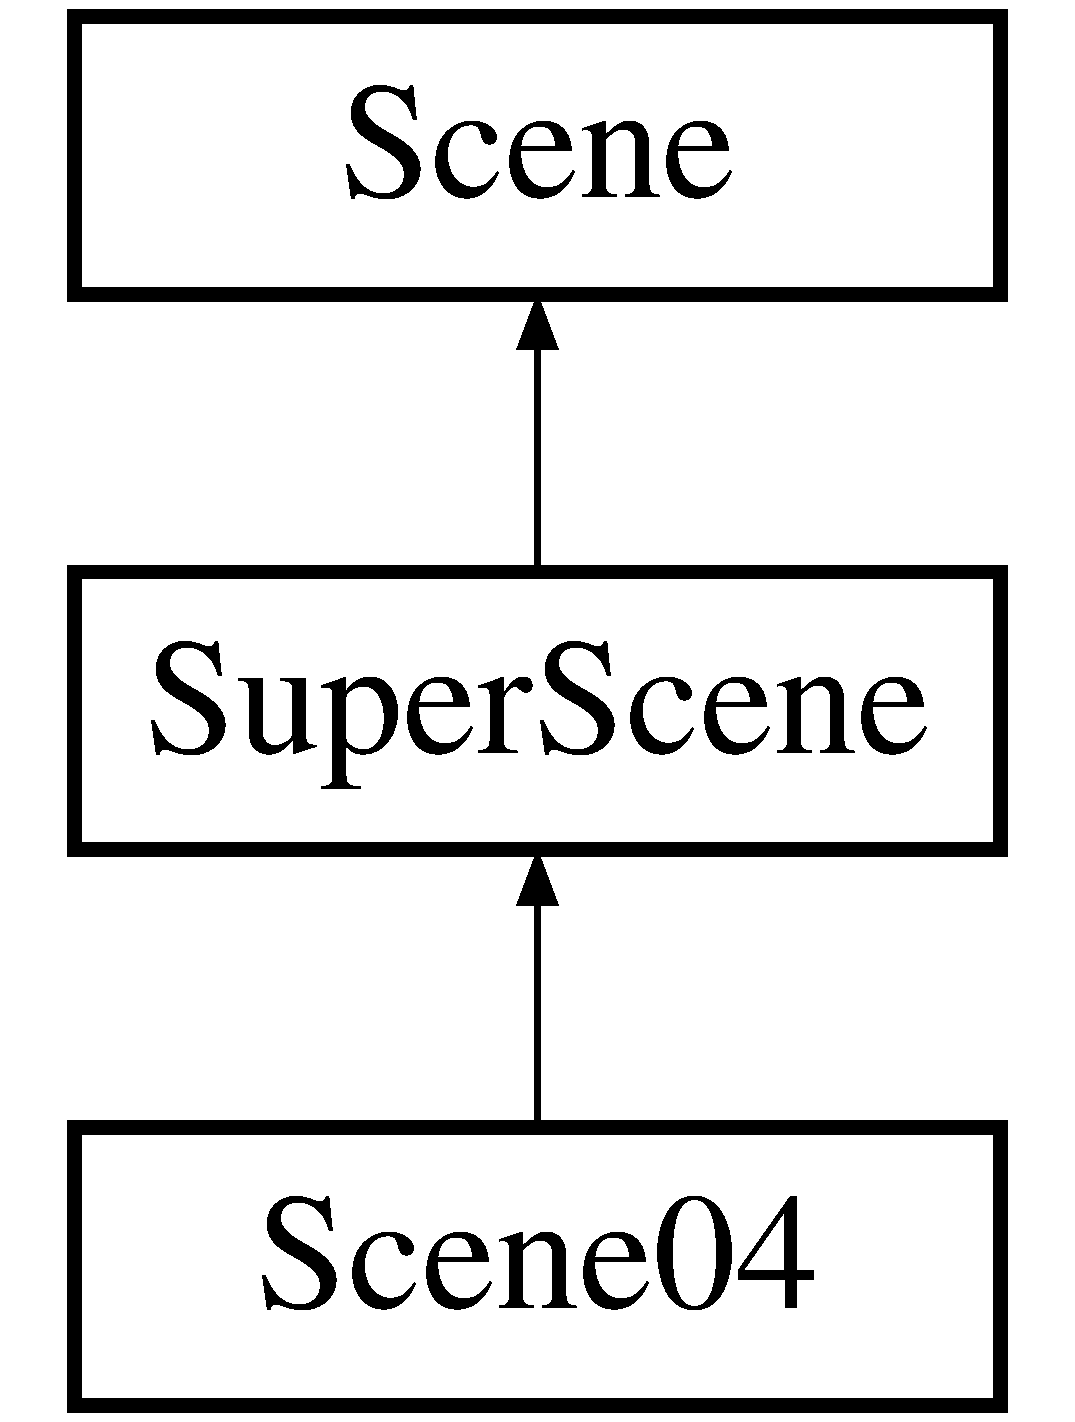
\includegraphics[height=3.000000cm]{class_scene04}
\end{center}
\end{figure}
\subsection*{Public Member Functions}
\begin{DoxyCompactItemize}
\item 
\hyperlink{class_scene04_acc9abfd3e2a3bd624ca980ac0589e48d}{Scene04} ()
\item 
\mbox{\Hypertarget{class_scene04_a492ca1581c60922f7c8959af8adb3035}\label{class_scene04_a492ca1581c60922f7c8959af8adb3035}} 
virtual void {\bfseries update} (float delta\+Time)
\end{DoxyCompactItemize}
\subsection*{Additional Inherited Members}


\subsection{Detailed Description}
This file is part of a demo that shows how to use R\+T2D, a 2D Open\+GL framework.


\begin{DoxyItemize}
\item Copyright 2015 Rik Teerling \href{mailto:rik@onandoffables.com}{\tt rik@onandoffables.\+com}
\begin{DoxyItemize}
\item Initial commit 
\end{DoxyItemize}
\end{DoxyItemize}

\subsection{Constructor \& Destructor Documentation}
\mbox{\Hypertarget{class_scene04_acc9abfd3e2a3bd624ca980ac0589e48d}\label{class_scene04_acc9abfd3e2a3bd624ca980ac0589e48d}} 
\index{Scene04@{Scene04}!Scene04@{Scene04}}
\index{Scene04@{Scene04}!Scene04@{Scene04}}
\subsubsection{\texorpdfstring{Scene04()}{Scene04()}}
{\footnotesize\ttfamily Scene04\+::\+Scene04 (\begin{DoxyParamCaption}{ }\end{DoxyParamCaption})}

This file is part of a demo that shows how to use R\+T2D, a 2D Open\+GL framework.


\begin{DoxyItemize}
\item Copyright 2015 Rik Teerling \href{mailto:rik@onandoffables.com}{\tt rik@onandoffables.\+com}
\begin{DoxyItemize}
\item Initial commit 
\end{DoxyItemize}
\end{DoxyItemize}

The documentation for this class was generated from the following files\+:\begin{DoxyCompactItemize}
\item 
scene04.\+h\item 
scene04.\+cpp\end{DoxyCompactItemize}

\hypertarget{class_scene05}{}\section{Scene05 Class Reference}
\label{class_scene05}\index{Scene05@{Scene05}}


{\ttfamily \#include $<$scene05.\+h$>$}

Inheritance diagram for Scene05\+:\begin{figure}[H]
\begin{center}
\leavevmode
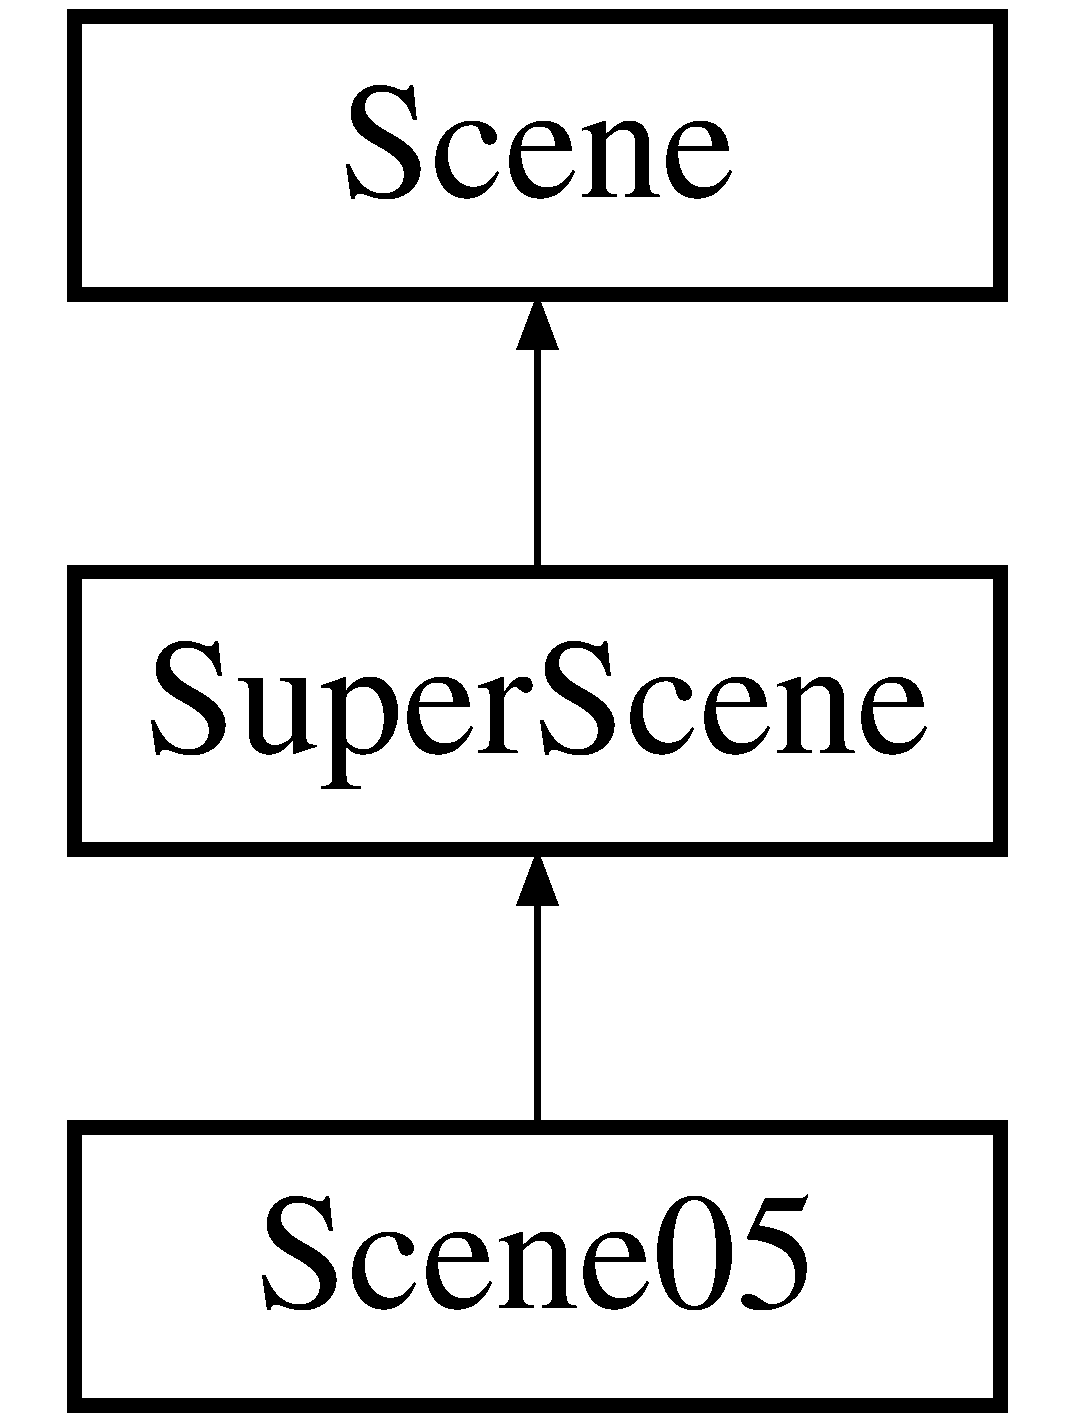
\includegraphics[height=3.000000cm]{class_scene05}
\end{center}
\end{figure}
\subsection*{Public Member Functions}
\begin{DoxyCompactItemize}
\item 
\hyperlink{class_scene05_af2500fef131d671d494dd87453b6f9a6}{Scene05} ()
\item 
\mbox{\Hypertarget{class_scene05_a130eb27e91bce97625df565cf7054b3f}\label{class_scene05_a130eb27e91bce97625df565cf7054b3f}} 
virtual void {\bfseries update} (float delta\+Time)
\end{DoxyCompactItemize}
\subsection*{Additional Inherited Members}


\subsection{Detailed Description}
This file is part of a demo that shows how to use R\+T2D, a 2D Open\+GL framework.


\begin{DoxyItemize}
\item Copyright 2015 Rik Teerling \href{mailto:rik@onandoffables.com}{\tt rik@onandoffables.\+com}
\begin{DoxyItemize}
\item Initial commit 
\end{DoxyItemize}
\end{DoxyItemize}

\subsection{Constructor \& Destructor Documentation}
\mbox{\Hypertarget{class_scene05_af2500fef131d671d494dd87453b6f9a6}\label{class_scene05_af2500fef131d671d494dd87453b6f9a6}} 
\index{Scene05@{Scene05}!Scene05@{Scene05}}
\index{Scene05@{Scene05}!Scene05@{Scene05}}
\subsubsection{\texorpdfstring{Scene05()}{Scene05()}}
{\footnotesize\ttfamily Scene05\+::\+Scene05 (\begin{DoxyParamCaption}{ }\end{DoxyParamCaption})}

This file is part of a demo that shows how to use R\+T2D, a 2D Open\+GL framework.


\begin{DoxyItemize}
\item Copyright 2015 Rik Teerling \href{mailto:rik@onandoffables.com}{\tt rik@onandoffables.\+com}
\begin{DoxyItemize}
\item Initial commit 
\end{DoxyItemize}
\end{DoxyItemize}

The documentation for this class was generated from the following files\+:\begin{DoxyCompactItemize}
\item 
scene05.\+h\item 
scene05.\+cpp\end{DoxyCompactItemize}

\hypertarget{class_scene06}{}\section{Scene06 Class Reference}
\label{class_scene06}\index{Scene06@{Scene06}}


{\ttfamily \#include $<$scene06.\+h$>$}

Inheritance diagram for Scene06\+:\begin{figure}[H]
\begin{center}
\leavevmode
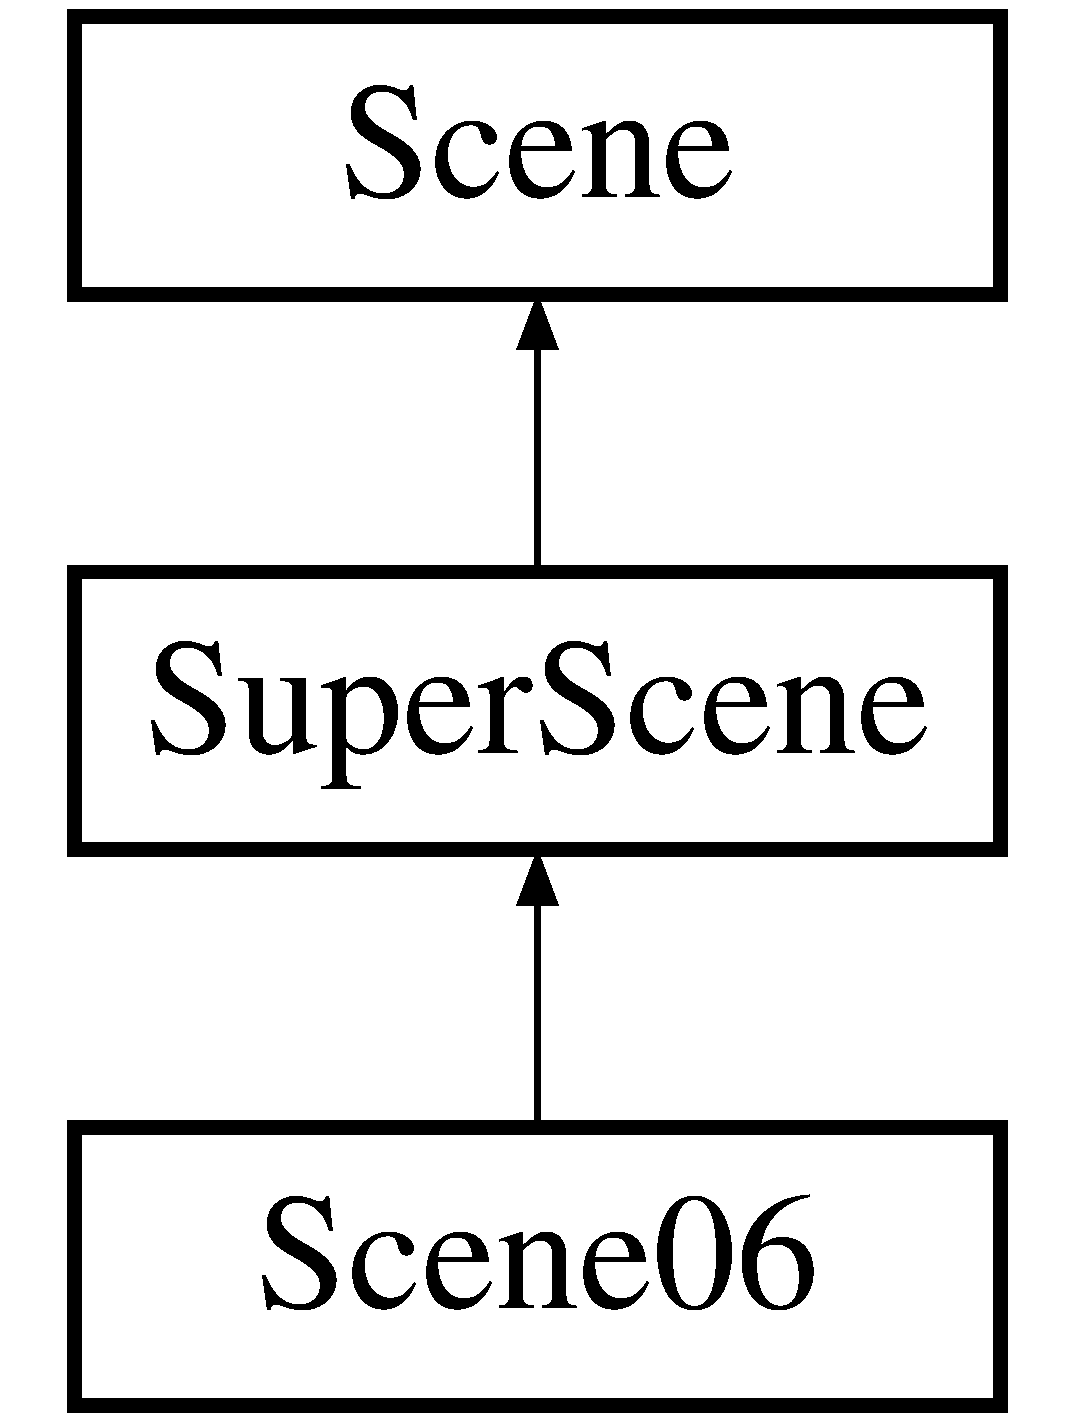
\includegraphics[height=3.000000cm]{class_scene06}
\end{center}
\end{figure}
\subsection*{Public Member Functions}
\begin{DoxyCompactItemize}
\item 
\hyperlink{class_scene06_a0fe3319d082e484405ec497d809f20eb}{Scene06} ()
\item 
\mbox{\Hypertarget{class_scene06_af8bfea85334f834952d409b8b85084fe}\label{class_scene06_af8bfea85334f834952d409b8b85084fe}} 
virtual void {\bfseries update} (float delta\+Time)
\end{DoxyCompactItemize}
\subsection*{Additional Inherited Members}


\subsection{Detailed Description}
This file is part of a demo that shows how to use R\+T2D, a 2D Open\+GL framework.


\begin{DoxyItemize}
\item Copyright 2015 Rik Teerling \href{mailto:rik@onandoffables.com}{\tt rik@onandoffables.\+com}
\begin{DoxyItemize}
\item Initial commit 
\end{DoxyItemize}
\end{DoxyItemize}

\subsection{Constructor \& Destructor Documentation}
\mbox{\Hypertarget{class_scene06_a0fe3319d082e484405ec497d809f20eb}\label{class_scene06_a0fe3319d082e484405ec497d809f20eb}} 
\index{Scene06@{Scene06}!Scene06@{Scene06}}
\index{Scene06@{Scene06}!Scene06@{Scene06}}
\subsubsection{\texorpdfstring{Scene06()}{Scene06()}}
{\footnotesize\ttfamily Scene06\+::\+Scene06 (\begin{DoxyParamCaption}{ }\end{DoxyParamCaption})}

This file is part of a demo that shows how to use R\+T2D, a 2D Open\+GL framework.


\begin{DoxyItemize}
\item Copyright 2015 Rik Teerling \href{mailto:rik@onandoffables.com}{\tt rik@onandoffables.\+com}
\begin{DoxyItemize}
\item Initial commit 
\end{DoxyItemize}
\end{DoxyItemize}

The documentation for this class was generated from the following files\+:\begin{DoxyCompactItemize}
\item 
scene06.\+h\item 
scene06.\+cpp\end{DoxyCompactItemize}

\hypertarget{class_scene06a}{}\section{Scene06a Class Reference}
\label{class_scene06a}\index{Scene06a@{Scene06a}}
Inheritance diagram for Scene06a\+:\begin{figure}[H]
\begin{center}
\leavevmode
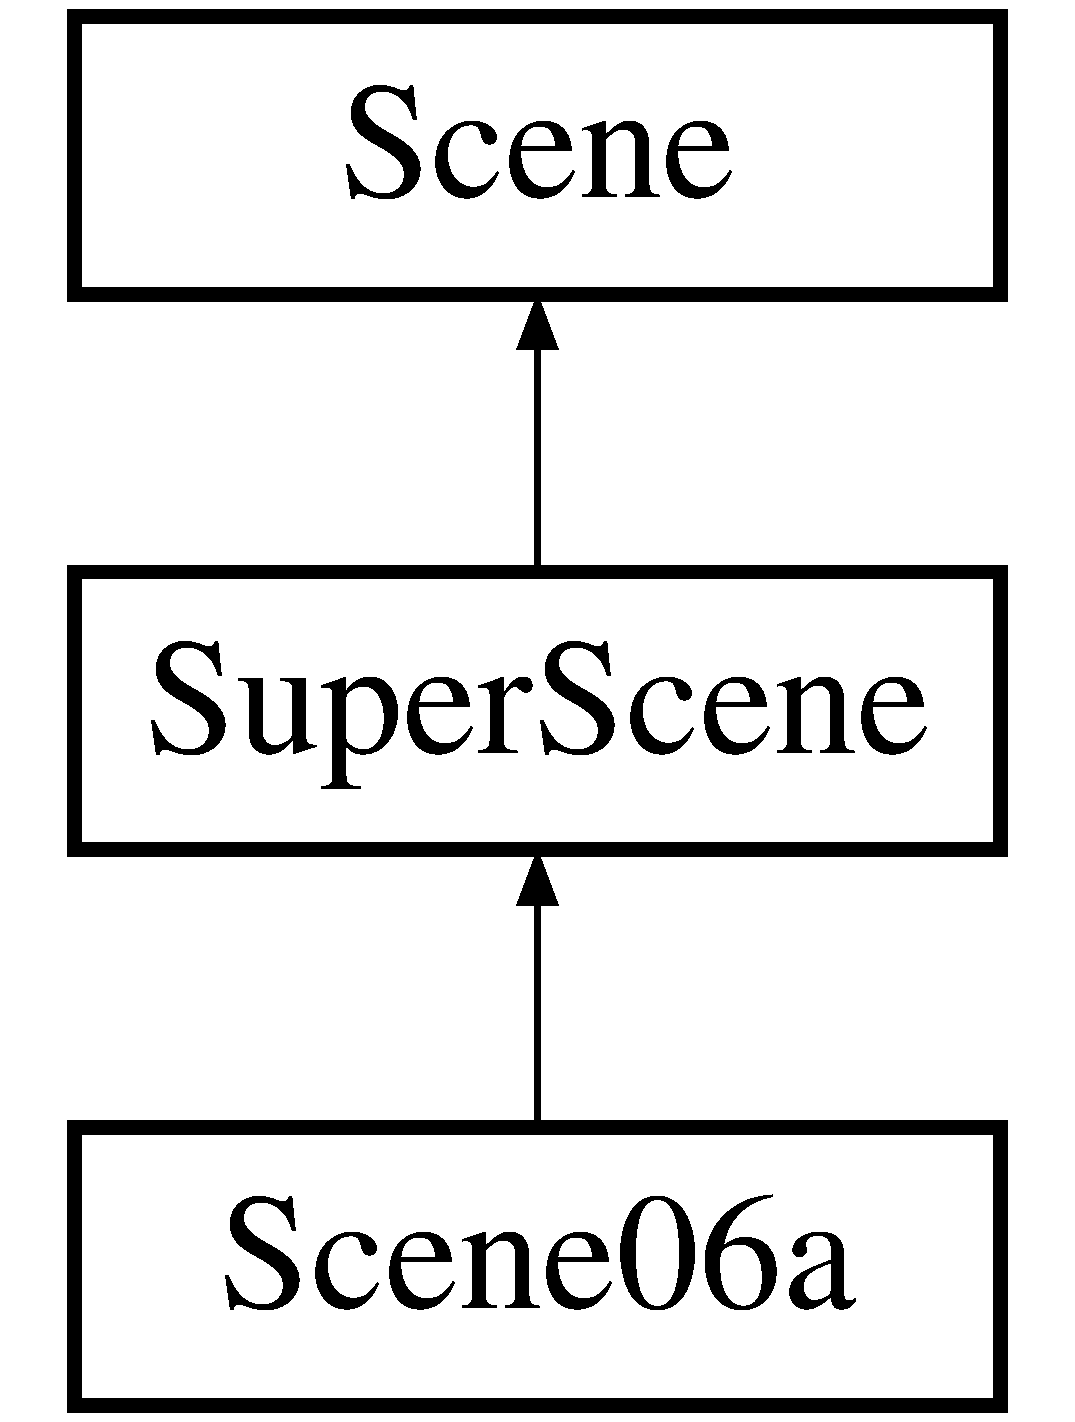
\includegraphics[height=3.000000cm]{class_scene06a}
\end{center}
\end{figure}
\subsection*{Public Member Functions}
\begin{DoxyCompactItemize}
\item 
\hyperlink{class_scene06a_aae1a94fddd7955e64c2cc8a1b670437d}{Scene06a} ()
\item 
\mbox{\Hypertarget{class_scene06a_ab7540d27c16b53f6a4aee09d12036ef4}\label{class_scene06a_ab7540d27c16b53f6a4aee09d12036ef4}} 
virtual void {\bfseries update} (float delta\+Time)
\end{DoxyCompactItemize}
\subsection*{Additional Inherited Members}


\subsection{Constructor \& Destructor Documentation}
\mbox{\Hypertarget{class_scene06a_aae1a94fddd7955e64c2cc8a1b670437d}\label{class_scene06a_aae1a94fddd7955e64c2cc8a1b670437d}} 
\index{Scene06a@{Scene06a}!Scene06a@{Scene06a}}
\index{Scene06a@{Scene06a}!Scene06a@{Scene06a}}
\subsubsection{\texorpdfstring{Scene06a()}{Scene06a()}}
{\footnotesize\ttfamily Scene06a\+::\+Scene06a (\begin{DoxyParamCaption}{ }\end{DoxyParamCaption})}

This file is part of a demo that shows how to use R\+T2D, a 2D Open\+GL framework.


\begin{DoxyItemize}
\item Copyright 2017 Rik Teerling \href{mailto:rik@onandoffables.com}{\tt rik@onandoffables.\+com}
\begin{DoxyItemize}
\item Initial commit 
\end{DoxyItemize}
\end{DoxyItemize}

The documentation for this class was generated from the following files\+:\begin{DoxyCompactItemize}
\item 
scene06a.\+h\item 
scene06a.\+cpp\end{DoxyCompactItemize}

\hypertarget{class_scene07}{}\section{Scene07 Class Reference}
\label{class_scene07}\index{Scene07@{Scene07}}
Inheritance diagram for Scene07\+:\begin{figure}[H]
\begin{center}
\leavevmode
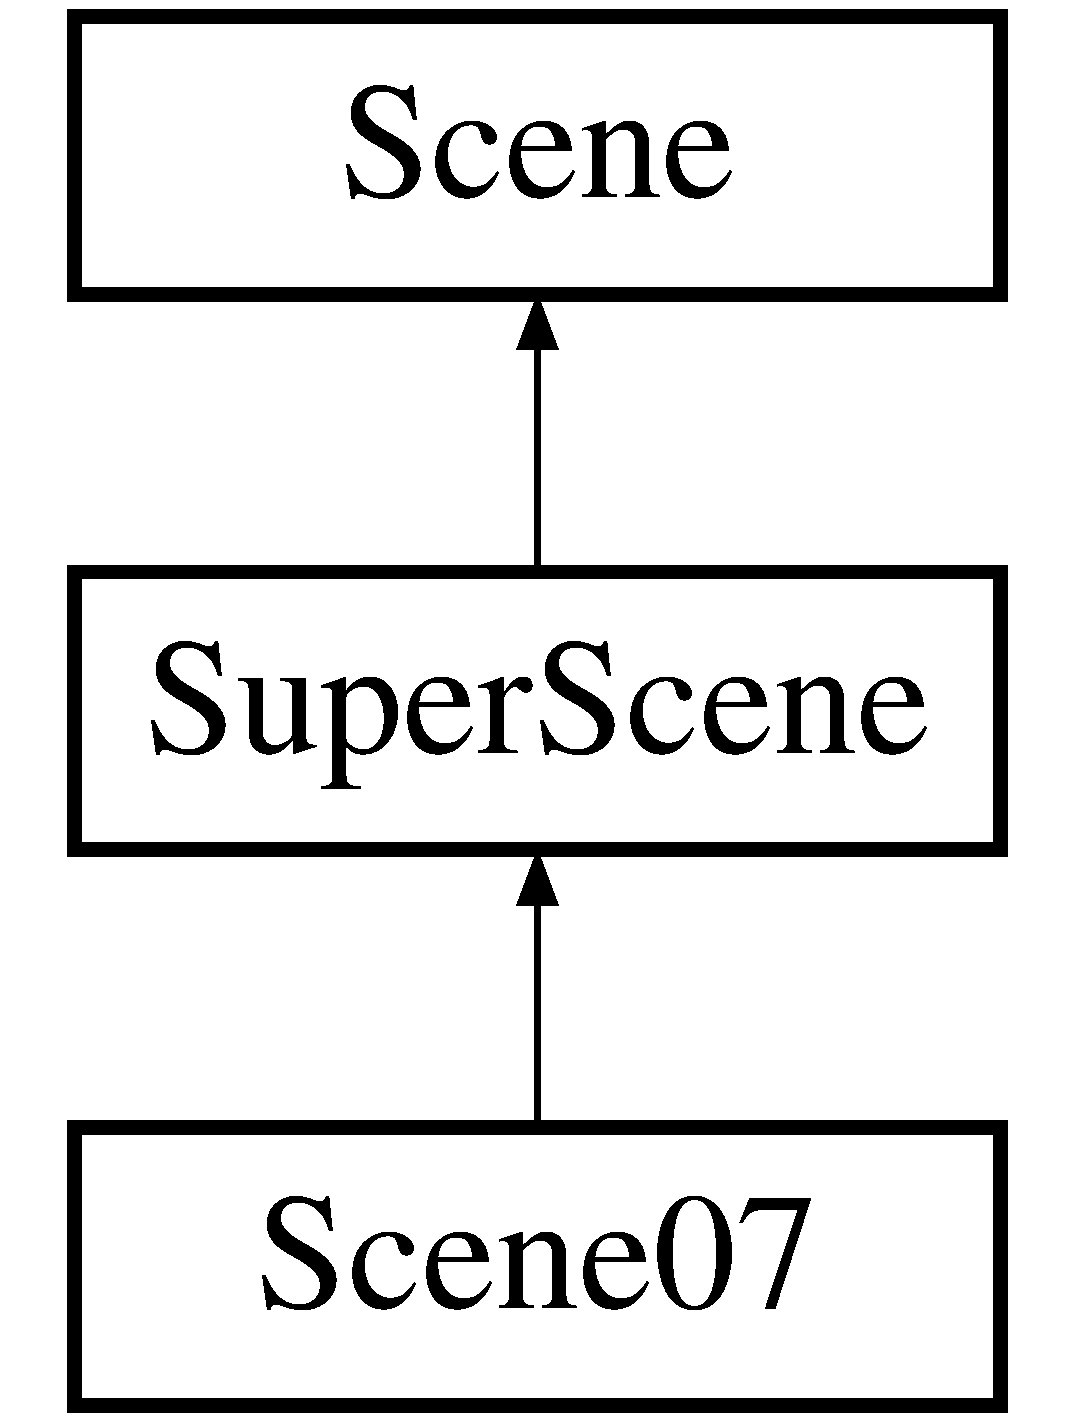
\includegraphics[height=3.000000cm]{class_scene07}
\end{center}
\end{figure}
\subsection*{Public Member Functions}
\begin{DoxyCompactItemize}
\item 
\hyperlink{class_scene07_a22c12ec7c0df5e38b289a459da70989b}{Scene07} ()
\item 
\mbox{\Hypertarget{class_scene07_a6fc20b8453f220586b73aed9af50afce}\label{class_scene07_a6fc20b8453f220586b73aed9af50afce}} 
virtual void {\bfseries update} (float delta\+Time)
\end{DoxyCompactItemize}
\subsection*{Additional Inherited Members}


\subsection{Constructor \& Destructor Documentation}
\mbox{\Hypertarget{class_scene07_a22c12ec7c0df5e38b289a459da70989b}\label{class_scene07_a22c12ec7c0df5e38b289a459da70989b}} 
\index{Scene07@{Scene07}!Scene07@{Scene07}}
\index{Scene07@{Scene07}!Scene07@{Scene07}}
\subsubsection{\texorpdfstring{Scene07()}{Scene07()}}
{\footnotesize\ttfamily Scene07\+::\+Scene07 (\begin{DoxyParamCaption}{ }\end{DoxyParamCaption})}

This file is part of a demo that shows how to use R\+T2D, a 2D Open\+GL framework.


\begin{DoxyItemize}
\item Copyright 2015 Rik Teerling \href{mailto:rik@onandoffables.com}{\tt rik@onandoffables.\+com}
\begin{DoxyItemize}
\item Initial commit 
\end{DoxyItemize}
\end{DoxyItemize}

The documentation for this class was generated from the following files\+:\begin{DoxyCompactItemize}
\item 
scene07.\+h\item 
scene07.\+cpp\end{DoxyCompactItemize}

\hypertarget{class_scene08}{}\section{Scene08 Class Reference}
\label{class_scene08}\index{Scene08@{Scene08}}
Inheritance diagram for Scene08\+:\begin{figure}[H]
\begin{center}
\leavevmode
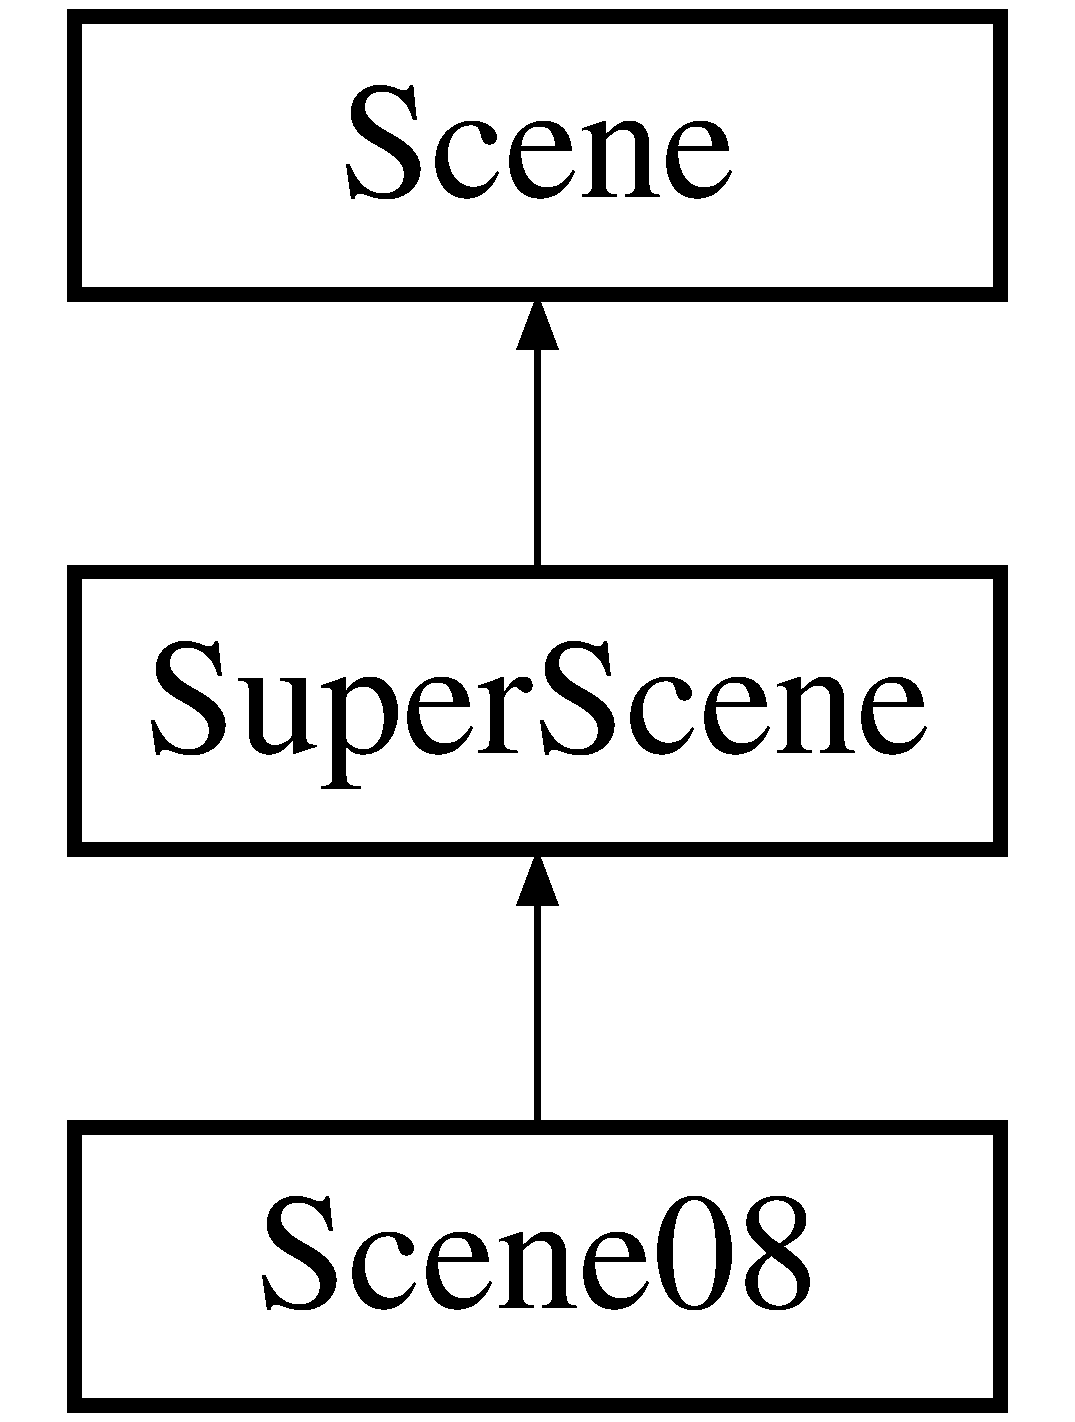
\includegraphics[height=3.000000cm]{class_scene08}
\end{center}
\end{figure}
\subsection*{Public Member Functions}
\begin{DoxyCompactItemize}
\item 
\hyperlink{class_scene08_aea86e2d7badbb0ddac6071ebeff068b1}{Scene08} ()
\item 
\mbox{\Hypertarget{class_scene08_ae20f71998a0e2d8ecbe4617d6fcf56ce}\label{class_scene08_ae20f71998a0e2d8ecbe4617d6fcf56ce}} 
virtual void {\bfseries update} (float delta\+Time)
\end{DoxyCompactItemize}
\subsection*{Additional Inherited Members}


\subsection{Constructor \& Destructor Documentation}
\mbox{\Hypertarget{class_scene08_aea86e2d7badbb0ddac6071ebeff068b1}\label{class_scene08_aea86e2d7badbb0ddac6071ebeff068b1}} 
\index{Scene08@{Scene08}!Scene08@{Scene08}}
\index{Scene08@{Scene08}!Scene08@{Scene08}}
\subsubsection{\texorpdfstring{Scene08()}{Scene08()}}
{\footnotesize\ttfamily Scene08\+::\+Scene08 (\begin{DoxyParamCaption}{ }\end{DoxyParamCaption})}

This file is part of a demo that shows how to use R\+T2D, a 2D Open\+GL framework.


\begin{DoxyItemize}
\item Copyright 2015 Rik Teerling \href{mailto:rik@onandoffables.com}{\tt rik@onandoffables.\+com}
\begin{DoxyItemize}
\item Initial commit 
\end{DoxyItemize}
\end{DoxyItemize}

The documentation for this class was generated from the following files\+:\begin{DoxyCompactItemize}
\item 
scene08.\+h\item 
scene08.\+cpp\end{DoxyCompactItemize}

\hypertarget{class_scene09}{}\section{Scene09 Class Reference}
\label{class_scene09}\index{Scene09@{Scene09}}


{\ttfamily \#include $<$scene09.\+h$>$}

Inheritance diagram for Scene09\+:\begin{figure}[H]
\begin{center}
\leavevmode
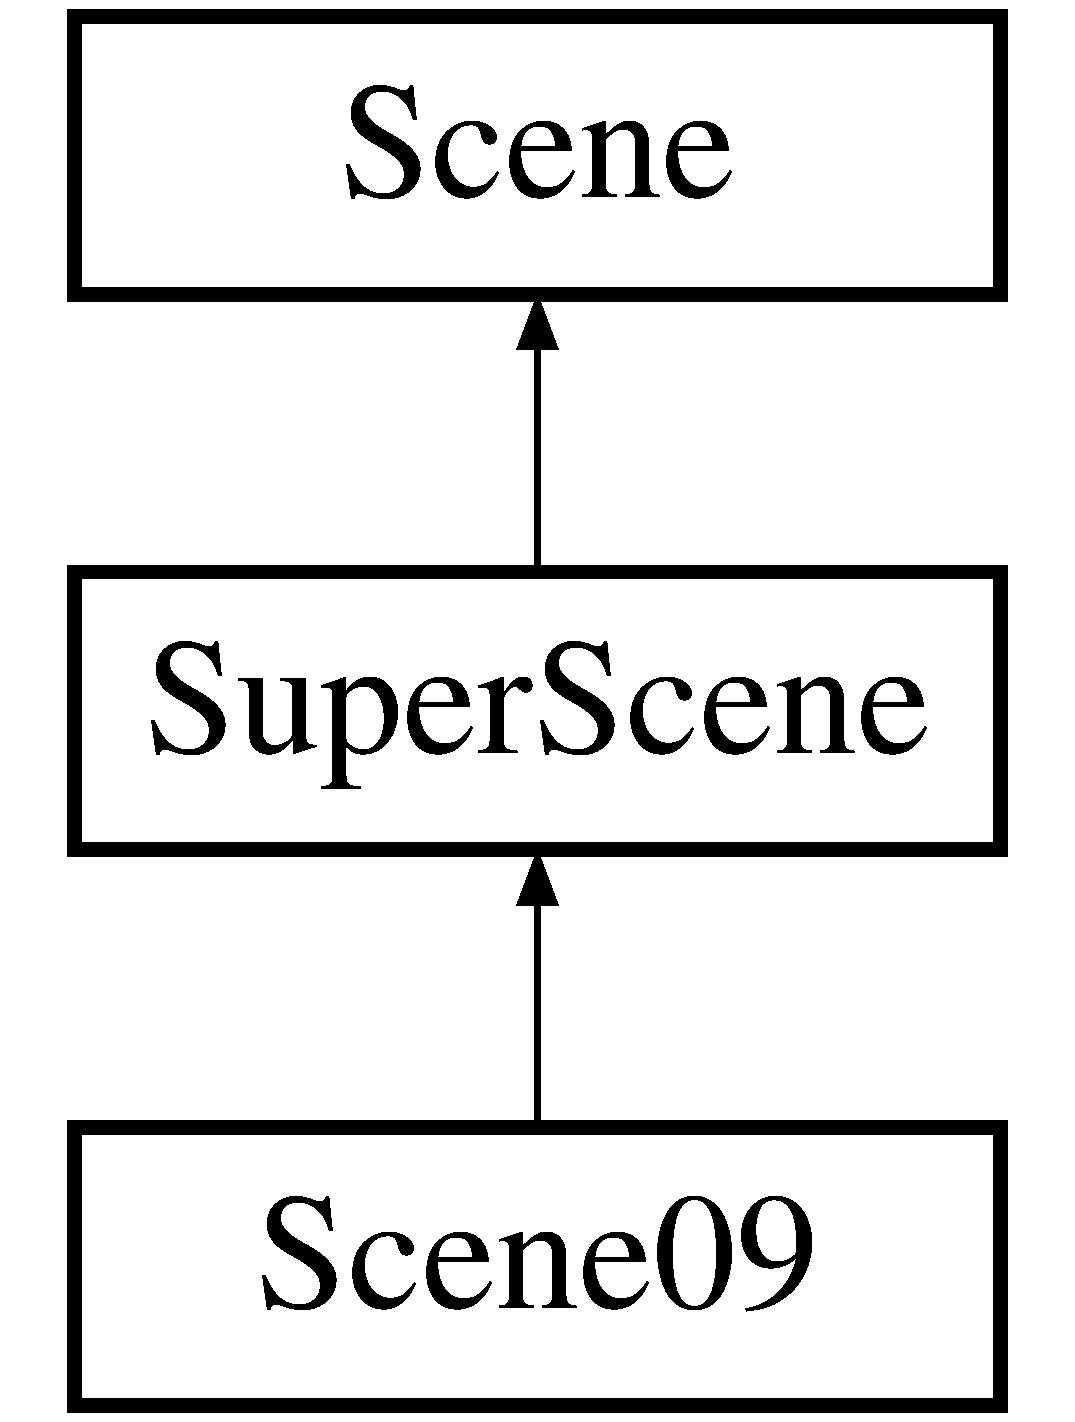
\includegraphics[height=3.000000cm]{class_scene09}
\end{center}
\end{figure}
\subsection*{Public Member Functions}
\begin{DoxyCompactItemize}
\item 
\hyperlink{class_scene09_a983b7890f9713f0c5f1e0aaa4e294e65}{Scene09} ()
\item 
\mbox{\Hypertarget{class_scene09_a6f138d71986fa190b38299e0f5277651}\label{class_scene09_a6f138d71986fa190b38299e0f5277651}} 
virtual void {\bfseries update} (float delta\+Time)
\end{DoxyCompactItemize}
\subsection*{Additional Inherited Members}


\subsection{Detailed Description}
This file is part of a demo that shows how to use R\+T2D, a 2D Open\+GL framework.


\begin{DoxyItemize}
\item Copyright 2015 Rik Teerling \href{mailto:rik@onandoffables.com}{\tt rik@onandoffables.\+com}
\begin{DoxyItemize}
\item Initial commit 
\end{DoxyItemize}
\end{DoxyItemize}

\subsection{Constructor \& Destructor Documentation}
\mbox{\Hypertarget{class_scene09_a983b7890f9713f0c5f1e0aaa4e294e65}\label{class_scene09_a983b7890f9713f0c5f1e0aaa4e294e65}} 
\index{Scene09@{Scene09}!Scene09@{Scene09}}
\index{Scene09@{Scene09}!Scene09@{Scene09}}
\subsubsection{\texorpdfstring{Scene09()}{Scene09()}}
{\footnotesize\ttfamily Scene09\+::\+Scene09 (\begin{DoxyParamCaption}{ }\end{DoxyParamCaption})}

This file is part of a demo that shows how to use R\+T2D, a 2D Open\+GL framework.


\begin{DoxyItemize}
\item Copyright 2015 Rik Teerling \href{mailto:rik@onandoffables.com}{\tt rik@onandoffables.\+com}
\begin{DoxyItemize}
\item Initial commit 
\end{DoxyItemize}
\end{DoxyItemize}

The documentation for this class was generated from the following files\+:\begin{DoxyCompactItemize}
\item 
scene09.\+h\item 
scene09.\+cpp\end{DoxyCompactItemize}

\hypertarget{class_scene10}{}\section{Scene10 Class Reference}
\label{class_scene10}\index{Scene10@{Scene10}}


{\ttfamily \#include $<$scene10.\+h$>$}

Inheritance diagram for Scene10\+:\begin{figure}[H]
\begin{center}
\leavevmode
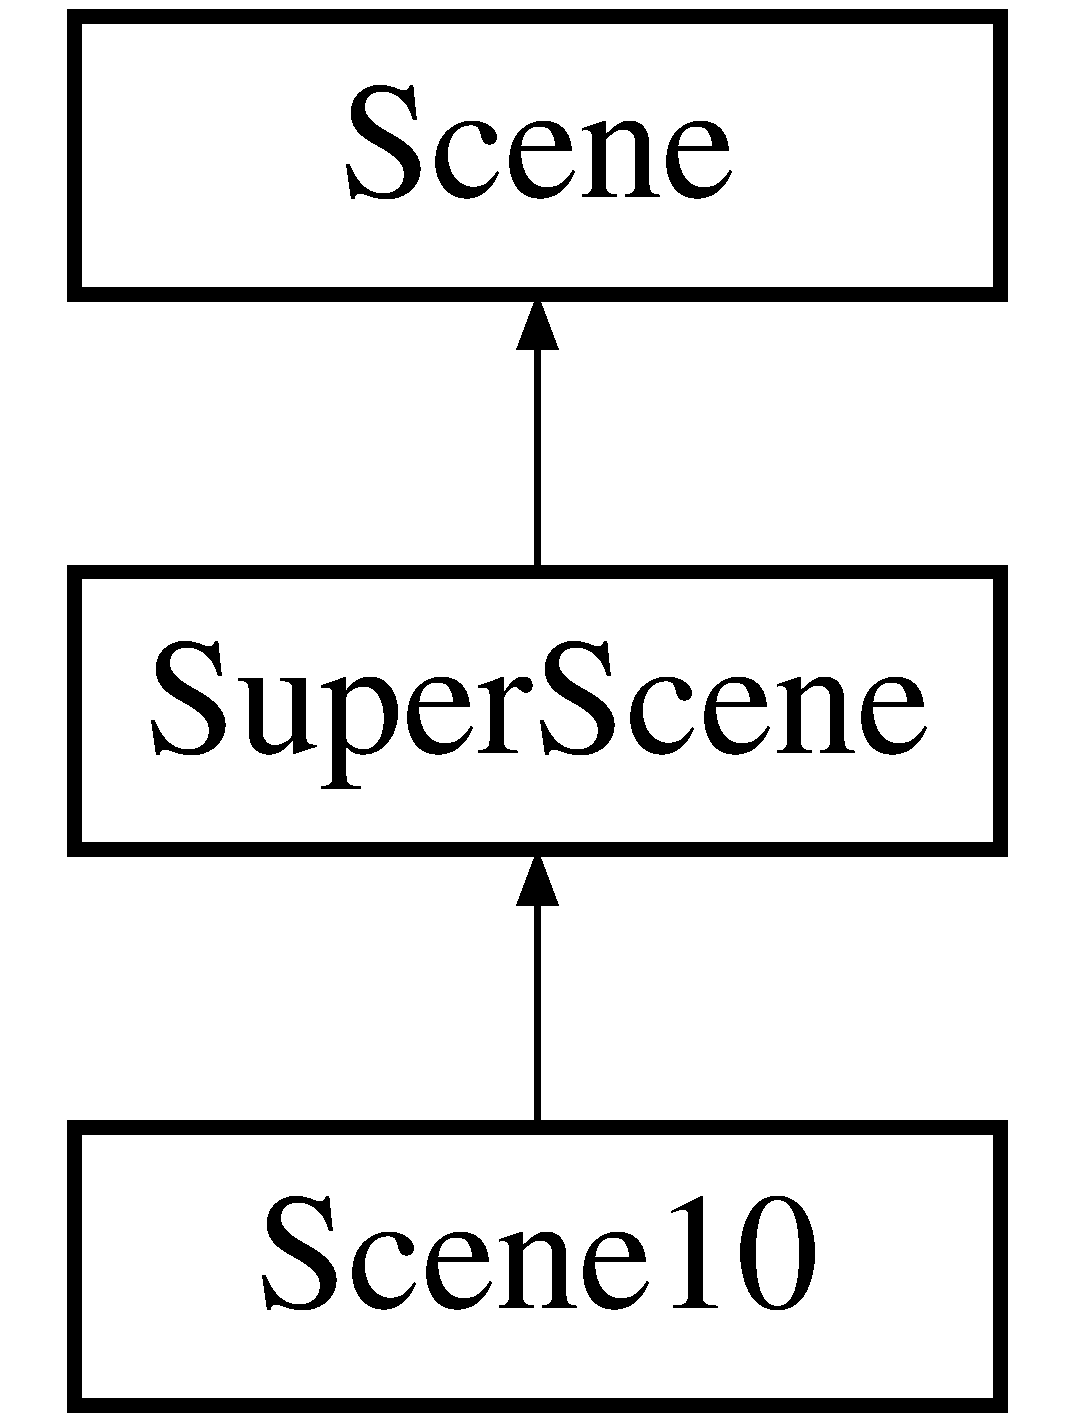
\includegraphics[height=3.000000cm]{class_scene10}
\end{center}
\end{figure}
\subsection*{Public Member Functions}
\begin{DoxyCompactItemize}
\item 
\hyperlink{class_scene10_adce71ede75c32dd246ec0d491dec531b}{Scene10} ()
\item 
\mbox{\Hypertarget{class_scene10_a8ce8f4d45625a7704bb8493317efc631}\label{class_scene10_a8ce8f4d45625a7704bb8493317efc631}} 
virtual void {\bfseries update} (float delta\+Time)
\end{DoxyCompactItemize}
\subsection*{Additional Inherited Members}


\subsection{Detailed Description}
This file is part of a demo that shows how to use R\+T2D, a 2D Open\+GL framework.


\begin{DoxyItemize}
\item Copyright 2015 Rik Teerling \href{mailto:rik@onandoffables.com}{\tt rik@onandoffables.\+com}
\begin{DoxyItemize}
\item Initial commit 
\end{DoxyItemize}
\end{DoxyItemize}

\subsection{Constructor \& Destructor Documentation}
\mbox{\Hypertarget{class_scene10_adce71ede75c32dd246ec0d491dec531b}\label{class_scene10_adce71ede75c32dd246ec0d491dec531b}} 
\index{Scene10@{Scene10}!Scene10@{Scene10}}
\index{Scene10@{Scene10}!Scene10@{Scene10}}
\subsubsection{\texorpdfstring{Scene10()}{Scene10()}}
{\footnotesize\ttfamily Scene10\+::\+Scene10 (\begin{DoxyParamCaption}{ }\end{DoxyParamCaption})}

This file is part of a demo that shows how to use R\+T2D, a 2D Open\+GL framework.


\begin{DoxyItemize}
\item Copyright 2015 Rik Teerling \href{mailto:rik@onandoffables.com}{\tt rik@onandoffables.\+com}
\begin{DoxyItemize}
\item Initial commit 
\end{DoxyItemize}
\end{DoxyItemize}

The documentation for this class was generated from the following files\+:\begin{DoxyCompactItemize}
\item 
scene10.\+h\item 
scene10.\+cpp\end{DoxyCompactItemize}

\hypertarget{class_scene11}{}\section{Scene11 Class Reference}
\label{class_scene11}\index{Scene11@{Scene11}}
Inheritance diagram for Scene11\+:\begin{figure}[H]
\begin{center}
\leavevmode
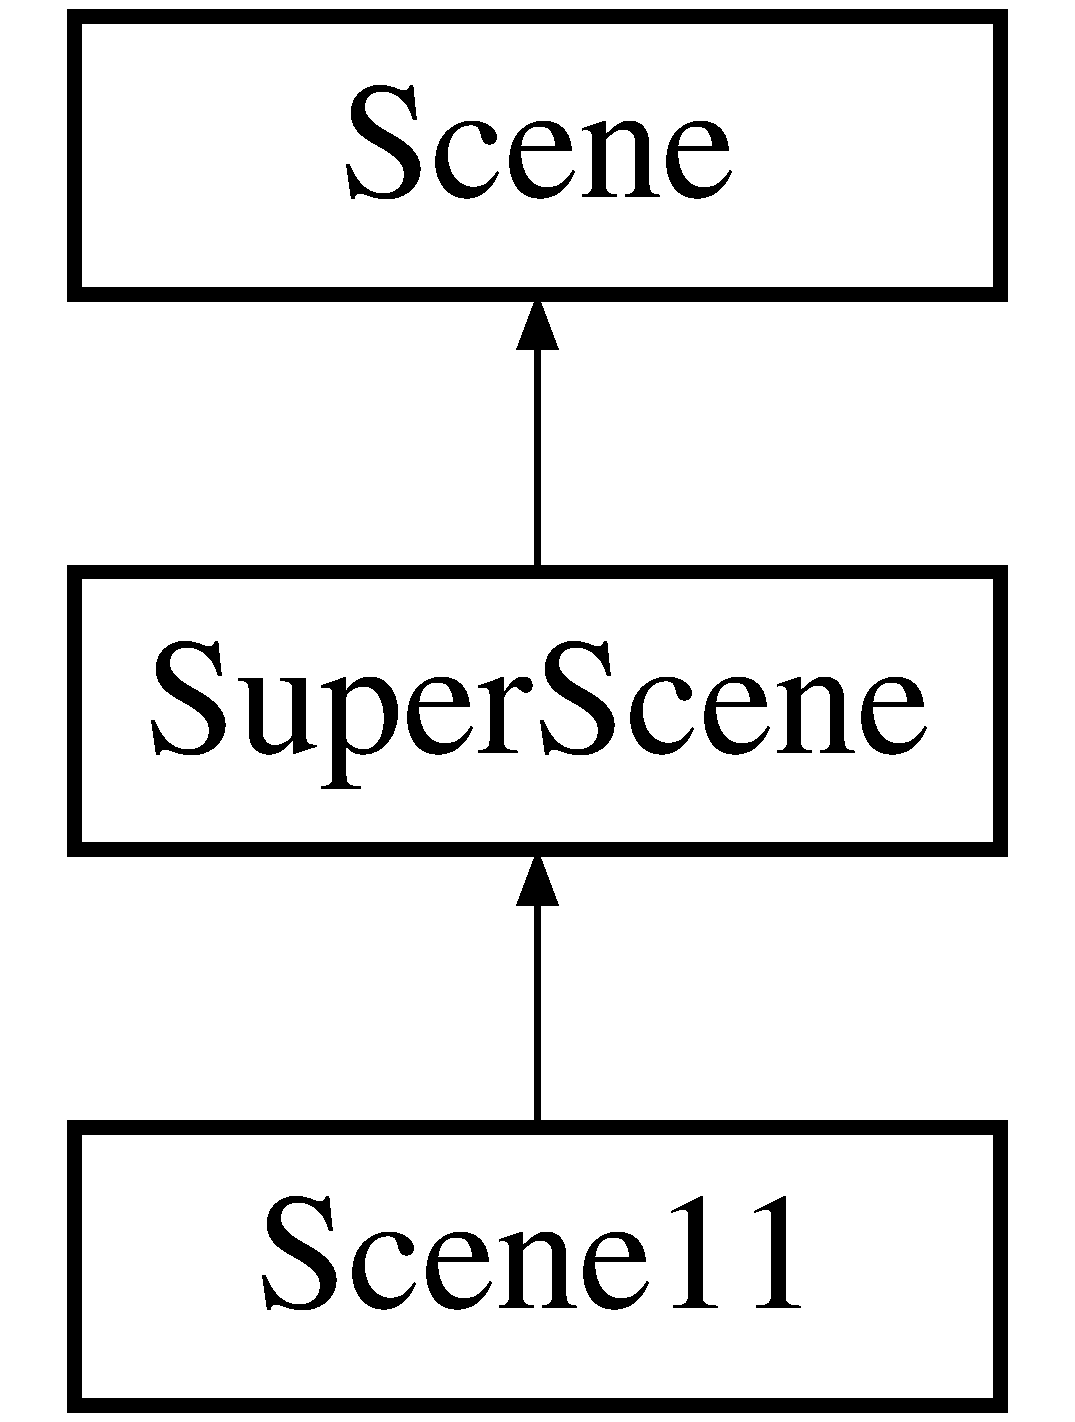
\includegraphics[height=3.000000cm]{class_scene11}
\end{center}
\end{figure}
\subsection*{Public Member Functions}
\begin{DoxyCompactItemize}
\item 
\hyperlink{class_scene11_a6a08d93da87ca19d59ddf98472c0b626}{Scene11} ()
\item 
\mbox{\Hypertarget{class_scene11_a17ec6c8da0b2402c79537d7eef7c63aa}\label{class_scene11_a17ec6c8da0b2402c79537d7eef7c63aa}} 
virtual void {\bfseries update} (float delta\+Time)
\end{DoxyCompactItemize}
\subsection*{Additional Inherited Members}


\subsection{Constructor \& Destructor Documentation}
\mbox{\Hypertarget{class_scene11_a6a08d93da87ca19d59ddf98472c0b626}\label{class_scene11_a6a08d93da87ca19d59ddf98472c0b626}} 
\index{Scene11@{Scene11}!Scene11@{Scene11}}
\index{Scene11@{Scene11}!Scene11@{Scene11}}
\subsubsection{\texorpdfstring{Scene11()}{Scene11()}}
{\footnotesize\ttfamily Scene11\+::\+Scene11 (\begin{DoxyParamCaption}{ }\end{DoxyParamCaption})}

This file is part of a demo that shows how to use R\+T2D, a 2D Open\+GL framework.


\begin{DoxyItemize}
\item Copyright 2016 Rik Teerling \href{mailto:rik@onandoffables.com}{\tt rik@onandoffables.\+com}
\begin{DoxyItemize}
\item Initial commit 
\end{DoxyItemize}
\end{DoxyItemize}

The documentation for this class was generated from the following files\+:\begin{DoxyCompactItemize}
\item 
scene11.\+h\item 
scene11.\+cpp\end{DoxyCompactItemize}

\hypertarget{class_scene12}{}\section{Scene12 Class Reference}
\label{class_scene12}\index{Scene12@{Scene12}}


{\ttfamily \#include $<$scene12.\+h$>$}

Inheritance diagram for Scene12\+:\begin{figure}[H]
\begin{center}
\leavevmode
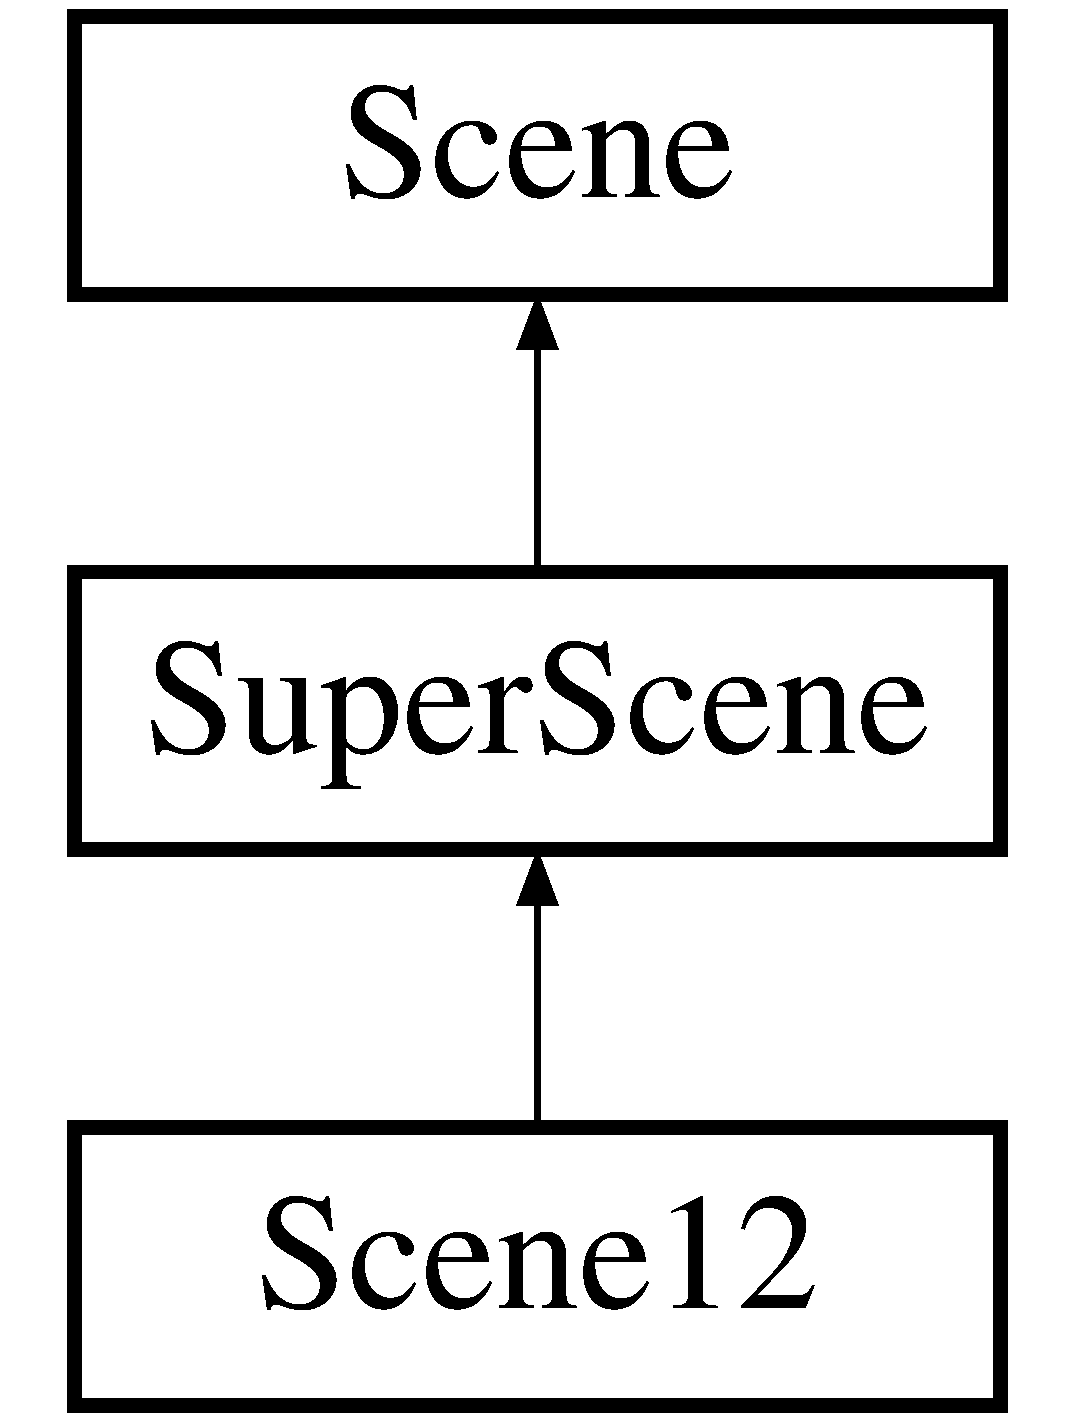
\includegraphics[height=3.000000cm]{class_scene12}
\end{center}
\end{figure}
\subsection*{Public Member Functions}
\begin{DoxyCompactItemize}
\item 
\hyperlink{class_scene12_aa060f8a7b4560c810120a82ebebfee3d}{Scene12} ()
\item 
\mbox{\Hypertarget{class_scene12_aac1be6b461b9290a457b528056fd8263}\label{class_scene12_aac1be6b461b9290a457b528056fd8263}} 
virtual void {\bfseries update} (float delta\+Time)
\end{DoxyCompactItemize}
\subsection*{Additional Inherited Members}


\subsection{Detailed Description}
This file is part of a demo that shows how to use R\+T2D, a 2D Open\+GL framework.


\begin{DoxyItemize}
\item Copyright 2016 Rik Teerling \href{mailto:rik@onandoffables.com}{\tt rik@onandoffables.\+com}
\begin{DoxyItemize}
\item Initial commit 
\end{DoxyItemize}
\end{DoxyItemize}

\subsection{Constructor \& Destructor Documentation}
\mbox{\Hypertarget{class_scene12_aa060f8a7b4560c810120a82ebebfee3d}\label{class_scene12_aa060f8a7b4560c810120a82ebebfee3d}} 
\index{Scene12@{Scene12}!Scene12@{Scene12}}
\index{Scene12@{Scene12}!Scene12@{Scene12}}
\subsubsection{\texorpdfstring{Scene12()}{Scene12()}}
{\footnotesize\ttfamily Scene12\+::\+Scene12 (\begin{DoxyParamCaption}{ }\end{DoxyParamCaption})}

This file is part of a demo that shows how to use R\+T2D, a 2D Open\+GL framework.


\begin{DoxyItemize}
\item Copyright 2016 Rik Teerling \href{mailto:rik@onandoffables.com}{\tt rik@onandoffables.\+com}
\begin{DoxyItemize}
\item Initial commit 
\end{DoxyItemize}
\end{DoxyItemize}

The documentation for this class was generated from the following files\+:\begin{DoxyCompactItemize}
\item 
scene12.\+h\item 
scene12.\+cpp\end{DoxyCompactItemize}

\hypertarget{class_scene13}{}\section{Scene13 Class Reference}
\label{class_scene13}\index{Scene13@{Scene13}}
Inheritance diagram for Scene13\+:\begin{figure}[H]
\begin{center}
\leavevmode
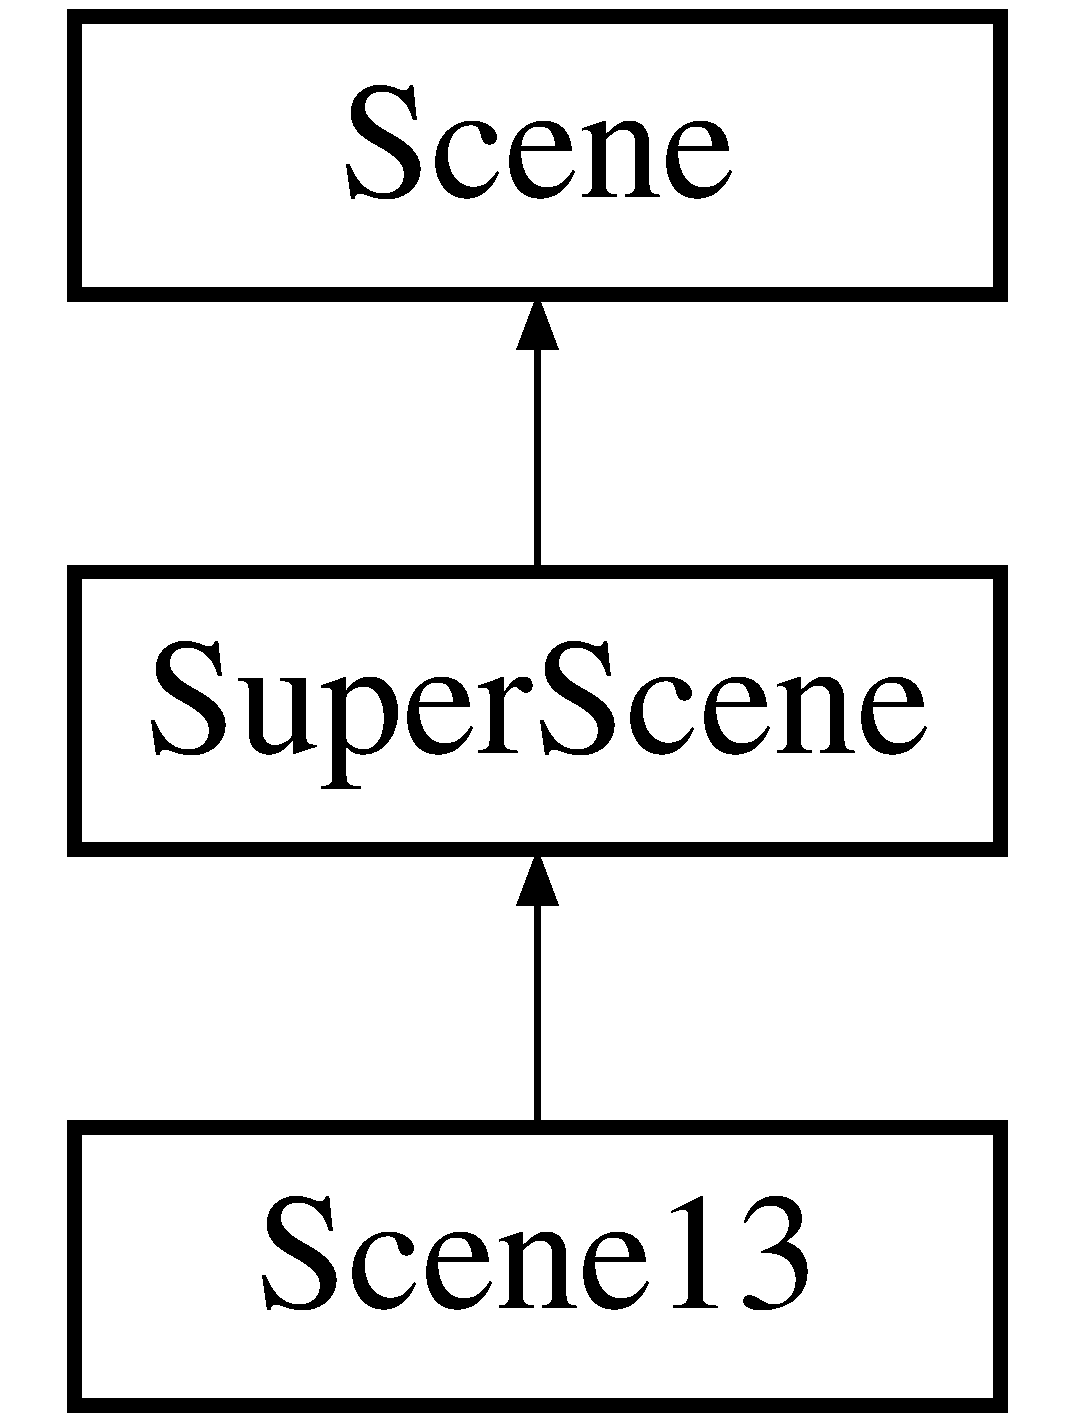
\includegraphics[height=3.000000cm]{class_scene13}
\end{center}
\end{figure}
\subsection*{Public Member Functions}
\begin{DoxyCompactItemize}
\item 
\hyperlink{class_scene13_a43fd3cea14e24f0b3e7d635d31e719bc}{Scene13} ()
\item 
\mbox{\Hypertarget{class_scene13_a3f6efaad7fadbecbf7718f004390b2d6}\label{class_scene13_a3f6efaad7fadbecbf7718f004390b2d6}} 
virtual void {\bfseries update} (float delta\+Time)
\end{DoxyCompactItemize}
\subsection*{Additional Inherited Members}


\subsection{Constructor \& Destructor Documentation}
\mbox{\Hypertarget{class_scene13_a43fd3cea14e24f0b3e7d635d31e719bc}\label{class_scene13_a43fd3cea14e24f0b3e7d635d31e719bc}} 
\index{Scene13@{Scene13}!Scene13@{Scene13}}
\index{Scene13@{Scene13}!Scene13@{Scene13}}
\subsubsection{\texorpdfstring{Scene13()}{Scene13()}}
{\footnotesize\ttfamily Scene13\+::\+Scene13 (\begin{DoxyParamCaption}{ }\end{DoxyParamCaption})}

This file is part of a demo that shows how to use R\+T2D, a 2D Open\+GL framework.


\begin{DoxyItemize}
\item Copyright 2016 Rik Teerling \href{mailto:rik@onandoffables.com}{\tt rik@onandoffables.\+com}
\begin{DoxyItemize}
\item Initial commit 
\end{DoxyItemize}
\end{DoxyItemize}

The documentation for this class was generated from the following files\+:\begin{DoxyCompactItemize}
\item 
scene13.\+h\item 
scene13.\+cpp\end{DoxyCompactItemize}

\hypertarget{class_scene14}{}\section{Scene14 Class Reference}
\label{class_scene14}\index{Scene14@{Scene14}}
Inheritance diagram for Scene14\+:\begin{figure}[H]
\begin{center}
\leavevmode
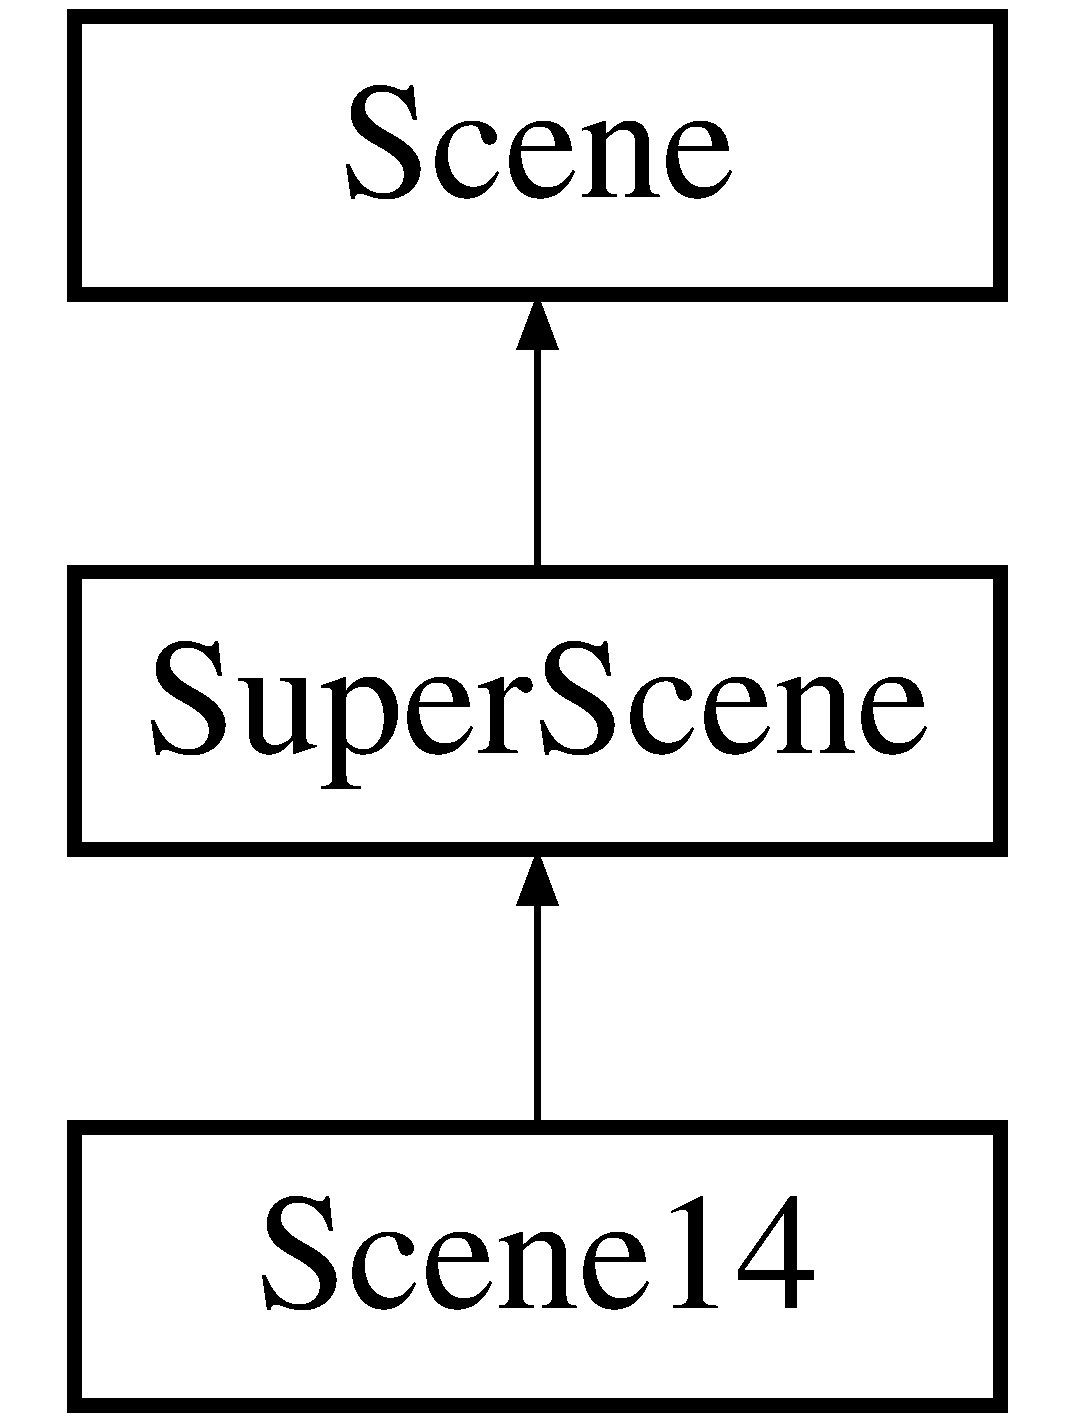
\includegraphics[height=3.000000cm]{class_scene14}
\end{center}
\end{figure}
\subsection*{Public Member Functions}
\begin{DoxyCompactItemize}
\item 
\hyperlink{class_scene14_a37a52d9fa06d04c8896b3ce15aede86a}{Scene14} ()
\item 
\mbox{\Hypertarget{class_scene14_a93f137ec994144f649cf7171f1f7bd93}\label{class_scene14_a93f137ec994144f649cf7171f1f7bd93}} 
virtual void {\bfseries update} (float delta\+Time)
\end{DoxyCompactItemize}
\subsection*{Additional Inherited Members}


\subsection{Constructor \& Destructor Documentation}
\mbox{\Hypertarget{class_scene14_a37a52d9fa06d04c8896b3ce15aede86a}\label{class_scene14_a37a52d9fa06d04c8896b3ce15aede86a}} 
\index{Scene14@{Scene14}!Scene14@{Scene14}}
\index{Scene14@{Scene14}!Scene14@{Scene14}}
\subsubsection{\texorpdfstring{Scene14()}{Scene14()}}
{\footnotesize\ttfamily Scene14\+::\+Scene14 (\begin{DoxyParamCaption}{ }\end{DoxyParamCaption})}

This file is part of a demo that shows how to use R\+T2D, a 2D Open\+GL framework.


\begin{DoxyItemize}
\item Copyright 2017 Rik Teerling \href{mailto:rik@onandoffables.com}{\tt rik@onandoffables.\+com}
\begin{DoxyItemize}
\item Initial commit 
\end{DoxyItemize}
\end{DoxyItemize}

The documentation for this class was generated from the following files\+:\begin{DoxyCompactItemize}
\item 
scene14.\+h\item 
scene14.\+cpp\end{DoxyCompactItemize}

\hypertarget{class_scene15}{}\section{Scene15 Class Reference}
\label{class_scene15}\index{Scene15@{Scene15}}


{\ttfamily \#include $<$scene15.\+h$>$}

Inheritance diagram for Scene15\+:\begin{figure}[H]
\begin{center}
\leavevmode
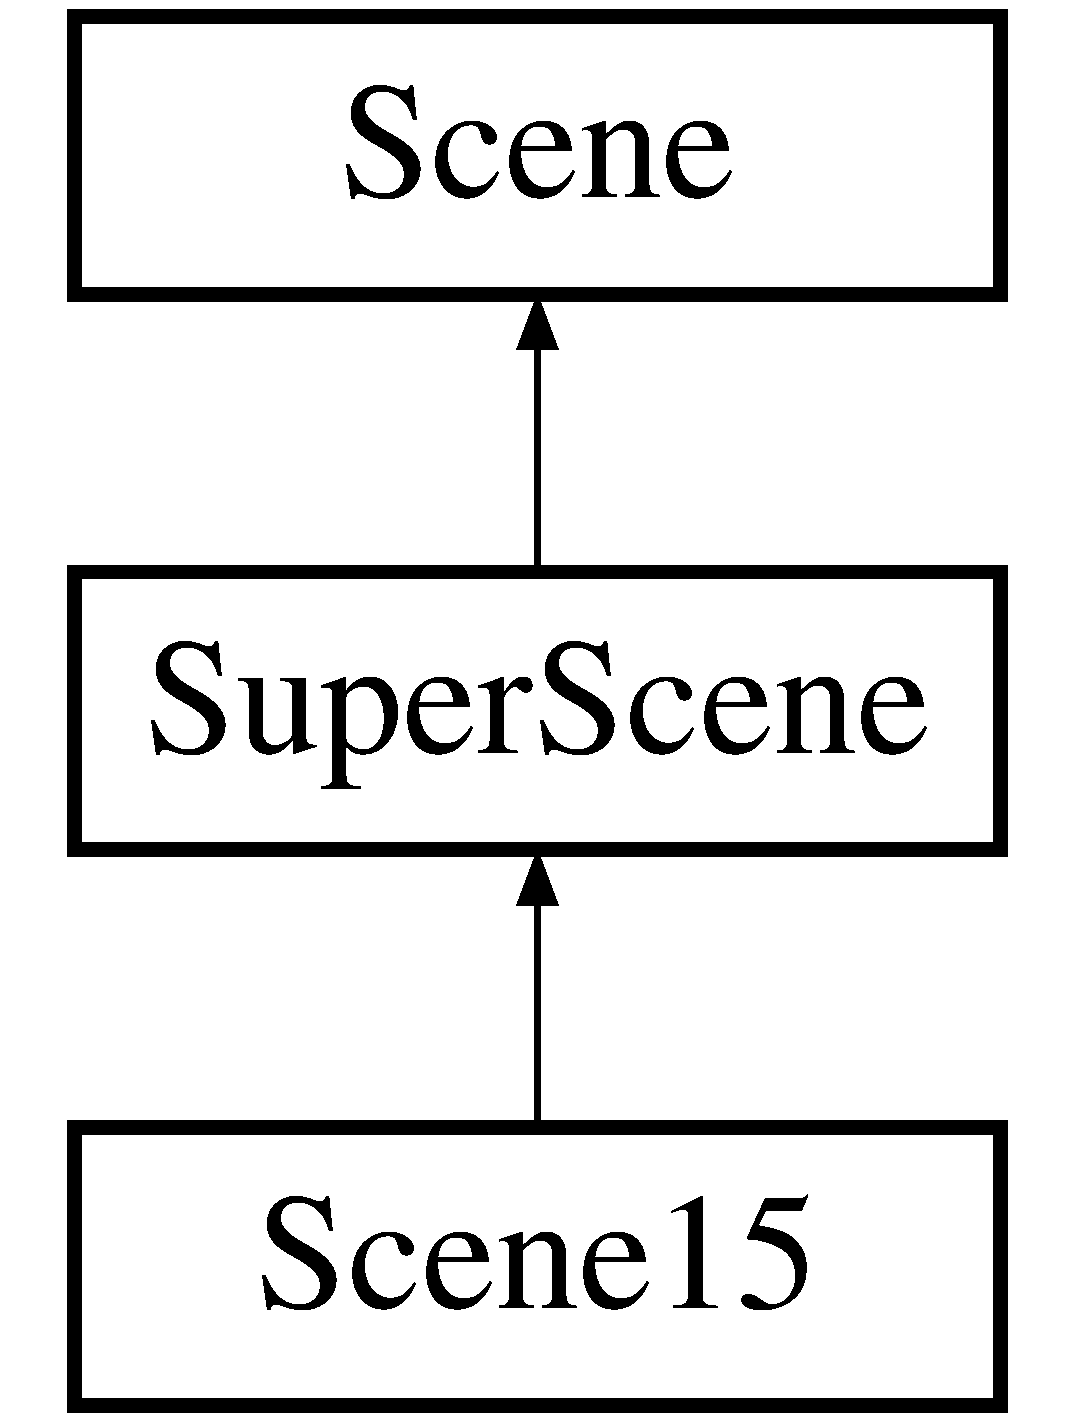
\includegraphics[height=3.000000cm]{class_scene15}
\end{center}
\end{figure}
\subsection*{Public Member Functions}
\begin{DoxyCompactItemize}
\item 
\hyperlink{class_scene15_aadba8e1ea9c1ab830e52be6d56cb5fea}{Scene15} ()
\item 
\mbox{\Hypertarget{class_scene15_a2d55c7e4ba97e1504d7e3e32ae680d5f}\label{class_scene15_a2d55c7e4ba97e1504d7e3e32ae680d5f}} 
virtual void {\bfseries update} (float delta\+Time)
\end{DoxyCompactItemize}
\subsection*{Additional Inherited Members}


\subsection{Detailed Description}
This file is part of a demo that shows how to use R\+T2D, a 2D Open\+GL framework.


\begin{DoxyItemize}
\item Copyright 2017 Rik Teerling \href{mailto:rik@onandoffables.com}{\tt rik@onandoffables.\+com}
\begin{DoxyItemize}
\item Initial commit 
\end{DoxyItemize}
\end{DoxyItemize}

\subsection{Constructor \& Destructor Documentation}
\mbox{\Hypertarget{class_scene15_aadba8e1ea9c1ab830e52be6d56cb5fea}\label{class_scene15_aadba8e1ea9c1ab830e52be6d56cb5fea}} 
\index{Scene15@{Scene15}!Scene15@{Scene15}}
\index{Scene15@{Scene15}!Scene15@{Scene15}}
\subsubsection{\texorpdfstring{Scene15()}{Scene15()}}
{\footnotesize\ttfamily Scene15\+::\+Scene15 (\begin{DoxyParamCaption}{ }\end{DoxyParamCaption})}

This file is part of a demo that shows how to use R\+T2D, a 2D Open\+GL framework.


\begin{DoxyItemize}
\item Copyright 2017 Rik Teerling \href{mailto:rik@onandoffables.com}{\tt rik@onandoffables.\+com}
\begin{DoxyItemize}
\item Initial commit 
\end{DoxyItemize}
\end{DoxyItemize}

The documentation for this class was generated from the following files\+:\begin{DoxyCompactItemize}
\item 
scene15.\+h\item 
scene15.\+cpp\end{DoxyCompactItemize}

\hypertarget{struct_s_i___animated_sprite}{}\section{S\+I\+\_\+\+Animated\+Sprite Struct Reference}
\label{struct_s_i___animated_sprite}\index{S\+I\+\_\+\+Animated\+Sprite@{S\+I\+\_\+\+Animated\+Sprite}}
\subsection*{Public Member Functions}
\begin{DoxyCompactItemize}
\item 
\mbox{\Hypertarget{struct_s_i___animated_sprite_aa12ad10e33a06d49e0811de67312b179}\label{struct_s_i___animated_sprite_aa12ad10e33a06d49e0811de67312b179}} 
void {\bfseries add\+Pixel\+Sprite} (\hyperlink{struct_pixel_sprite}{Pixel\+Sprite} ps)
\end{DoxyCompactItemize}
\subsection*{Public Attributes}
\begin{DoxyCompactItemize}
\item 
\mbox{\Hypertarget{struct_s_i___animated_sprite_a8d1e4690c159c9d1e12f0588b68abed7}\label{struct_s_i___animated_sprite_a8d1e4690c159c9d1e12f0588b68abed7}} 
Pointi {\bfseries position}
\item 
\mbox{\Hypertarget{struct_s_i___animated_sprite_a8951f2a3c0832be05e11f036f3497d12}\label{struct_s_i___animated_sprite_a8951f2a3c0832be05e11f036f3497d12}} 
Pointi {\bfseries velocity}
\item 
\mbox{\Hypertarget{struct_s_i___animated_sprite_a74dbd660f0abfdd5966617ab65ad7b0d}\label{struct_s_i___animated_sprite_a74dbd660f0abfdd5966617ab65ad7b0d}} 
std\+::vector$<$ \hyperlink{struct_pixel_sprite}{Pixel\+Sprite} $>$ {\bfseries frames}
\end{DoxyCompactItemize}


The documentation for this struct was generated from the following file\+:\begin{DoxyCompactItemize}
\item 
scene13.\+h\end{DoxyCompactItemize}

\hypertarget{class_super_scene}{}\section{Super\+Scene Class Reference}
\label{class_super_scene}\index{Super\+Scene@{Super\+Scene}}
Inheritance diagram for Super\+Scene\+:\begin{figure}[H]
\begin{center}
\leavevmode
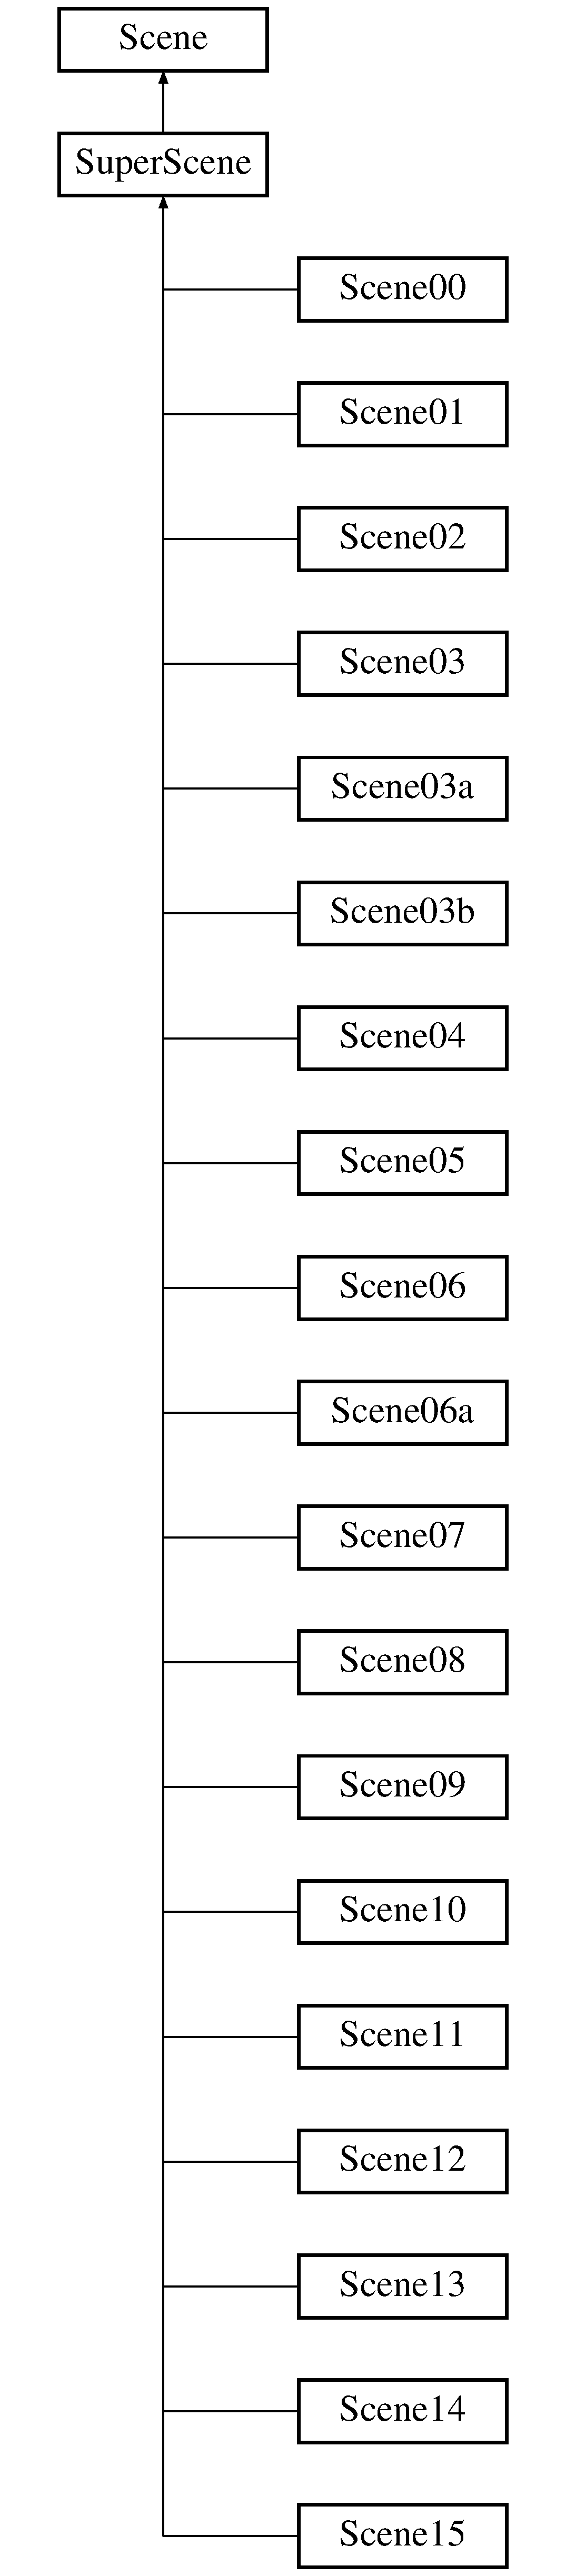
\includegraphics[height=12.000000cm]{class_super_scene}
\end{center}
\end{figure}
\subsection*{Public Member Functions}
\begin{DoxyCompactItemize}
\item 
\mbox{\Hypertarget{class_super_scene_a15f01dff85c3fd9933877b06b209c7ee}\label{class_super_scene_a15f01dff85c3fd9933877b06b209c7ee}} 
virtual void {\bfseries update} (float delta\+Time)
\item 
\mbox{\Hypertarget{class_super_scene_aa61d58308c7849a0a060c71cdbb6fac0}\label{class_super_scene_aa61d58308c7849a0a060c71cdbb6fac0}} 
void {\bfseries add\+Player} (\hyperlink{struct_player}{Player} $\ast$p)
\end{DoxyCompactItemize}
\subsection*{Static Public Attributes}
\begin{DoxyCompactItemize}
\item 
static int \hyperlink{class_super_scene_af98d73650372f31f17f19c02fde6f9be}{activescene} = 0
\end{DoxyCompactItemize}
\subsection*{Protected Member Functions}
\begin{DoxyCompactItemize}
\item 
\mbox{\Hypertarget{class_super_scene_ac0e2b1126702422c861d3f2cda5f1948}\label{class_super_scene_ac0e2b1126702422c861d3f2cda5f1948}} 
void {\bfseries move\+Camera} (float delta\+Time)
\end{DoxyCompactItemize}
\subsection*{Protected Attributes}
\begin{DoxyCompactItemize}
\item 
\mbox{\Hypertarget{class_super_scene_a4070e643a586cf61350ae18a0544165b}\label{class_super_scene_a4070e643a586cf61350ae18a0544165b}} 
unsigned int {\bfseries top\+\_\+layer}
\item 
\mbox{\Hypertarget{class_super_scene_a71b8a4d39ff9910f6b40f3cd110549d9}\label{class_super_scene_a71b8a4d39ff9910f6b40f3cd110549d9}} 
std\+::vector$<$ \hyperlink{class_basic_entity}{Basic\+Entity} $\ast$ $>$ {\bfseries layers}
\item 
\mbox{\Hypertarget{class_super_scene_a5a465432cc5223a4035e7bcefe26c07e}\label{class_super_scene_a5a465432cc5223a4035e7bcefe26c07e}} 
std\+::vector$<$ Text $\ast$ $>$ {\bfseries text}
\item 
\mbox{\Hypertarget{class_super_scene_a3888e131f19e0d6e74120c60cc89507a}\label{class_super_scene_a3888e131f19e0d6e74120c60cc89507a}} 
\hyperlink{struct_player}{Player} $\ast$ {\bfseries player}
\end{DoxyCompactItemize}


\subsection{Member Data Documentation}
\mbox{\Hypertarget{class_super_scene_af98d73650372f31f17f19c02fde6f9be}\label{class_super_scene_af98d73650372f31f17f19c02fde6f9be}} 
\index{Super\+Scene@{Super\+Scene}!activescene@{activescene}}
\index{activescene@{activescene}!Super\+Scene@{Super\+Scene}}
\subsubsection{\texorpdfstring{activescene}{activescene}}
{\footnotesize\ttfamily int Super\+Scene\+::activescene = 0\hspace{0.3cm}{\ttfamily [static]}}

This file is part of a demo that shows how to use R\+T2D, a 2D Open\+GL framework.


\begin{DoxyItemize}
\item Copyright 2015 Rik Teerling \href{mailto:rik@onandoffables.com}{\tt rik@onandoffables.\+com}
\begin{DoxyItemize}
\item Initial commit 
\end{DoxyItemize}
\end{DoxyItemize}

The documentation for this class was generated from the following files\+:\begin{DoxyCompactItemize}
\item 
superscene.\+h\item 
superscene.\+cpp\end{DoxyCompactItemize}

%--- End generated contents ---

% Index
\backmatter
\newpage
\phantomsection
\clearemptydoublepage
\addcontentsline{toc}{chapter}{Index}
\printindex

\end{document}
